% Intended LaTeX compiler: pdflatex
\documentclass[11pt]{report}
\usepackage[utf8]{inputenc}
\usepackage[T1]{fontenc}
\usepackage{graphicx}
\usepackage{amsmath}
\usepackage{amssymb}
\usepackage{hyperref}
\usepackage{booktabs}
\usepackage{biblatex}
%\usepackage{matlab-prettifier}

\date{\today\\\vspace*{2em}\emph{Unreviewed} notes for Prof. Smith's class. Use at own risk!}
\title{227-0689-00L: System Identification HS2023}
\author{Michele Zaffalon (Bruker BioSpin AG) \\ \\ Yannic Hofmann (ETHZ)}

\hypersetup{
  pdfauthor={Michele Zaffalon},
  pdftitle={System Identification},
  pdfkeywords={},
  pdfsubject={},
  pdfcreator={Emacs 29.1 (Org mode 9.6.6)},
  pdflang={English}}

\newcommand{\du}{\ensuremath{\mathrm{d}}}
% \newcommand{\bs}[1]{\boldsymbol{#1}}
% \newcommand{\bsrm}[1]{\boldsymbol{\mathrm{#1}}}
\newcommand{\II}{I}

\newcommand{\EE}[1]{\mathbb{E}\left\{#1\right\}}
\newcommand{\cov}[1]{\textrm{cov}\left(#1\right)}
\newcommand{\Bias}[1]{\textrm{Bias}\left(#1\right)}
\newcommand{\MSE}[1]{\textrm{MSE}\left(#1\right)}
\newcommand{\tr}[1]{\textrm{tr}\left(#1\right)}
\newcommand{\rank}[1]{\textrm{rank}\left(#1\right)}
\newcommand{\thetaLS}{\hat{\theta}_\textrm{LS}}
\newcommand{\thetaJS}{\hat{\theta}^\textrm{JS}}
\newcommand{\thetaR}{\hat{\theta}^\textrm{R}}

\newcommand{\taumax}{\tau_\text{max}}
\newcommand{\ejw}{e^{j\omega}}
\newcommand{\ejwn}[1][]{e^{j\omega_n#1}}
\newcommand{\emjwn}[1][]{e^{-j\omega_n#1}}


\addbibresource{notes.bib}

\begin{document}

\maketitle
\tableofcontents

% \include{stats}
\chapter{Least-Squares Estimation}
\label{chap:LS-estimation}

Consider a model
\begin{equation}
  \label{eq:LTI-with-noise}
  Y = \Phi\theta_0 + \epsilon
\end{equation}
where $Y = \begin{bmatrix}
  y_0 & \ldots && y_{N-1}
\end{bmatrix}^\top$ is a vector containing the measurements $\{y_0,\ldots, y_{N-1}\}$, $\Phi\in \mathbb{R}^{N\times p}$ is called the regressor and $\theta\in\mathbb{R}^p$ is the model parameter, the vector of $p$ unknown parameters to be estimated; $p$ is the model order.
The noise vector $\epsilon =
\begin{bmatrix}
  v_0 & \ldots & v_{N-1}
\end{bmatrix}^\top$ has zero mean $\EE{\epsilon}=0$ and covariance $\EE{\epsilon \epsilon^\top}=R$, a symmetric positive definite matrix.

The maximum likelihood (ML) probability\footnote{What is the expectation value of eq.~\eqref{eq:LS-problem}? Using eq.~\eqref{eq:thetaLS-estimate}, I \emph{think} the term $Y-\Phi\theta$ should be evaluated as
  \begin{equation*}
    Y-\Phi\thetaLS = \Phi\theta_0 + \epsilon - \Phi\theta_0 - \Phi K \Phi^\top R\epsilon = \left(I - \Phi K \Phi^\top R\right)\epsilon.
  \end{equation*}
  The average
  \begin{equation*}
    \EE{(Y - \Phi \thetaLS)^\top R^{-1} (Y - \Phi \thetaLS)} = \EE{\epsilon^\top\left(I - \Phi K \Phi^\top R\right)^\top R^{-1}\left(I - \Phi K \Phi^\top R\right)\epsilon}
  \end{equation*}
  but I do not know what the term $\EE{\epsilon^\top R^{-1}\epsilon}$ evaluates to. I expect this to be equal to $N$, at least this is what happens with an uncorrelated noise with constant variance.

  Note also that while the matrix $vv^\top$ has rank 1, the variance matrix $R$ for Gaussian distributed white noise is full rank because it is the sum of random vectors that span the whole space.} requires us to minimize
\begin{equation}
  \label{eq:LS-problem}
  (Y - \Phi \theta)^\top R^{-1} (Y - \Phi \theta) = ||C (Y - \Phi \theta)||_2^2
\end{equation}
where $C$ is the Cholesky decomposition of the symmetric positive definite matrix $C^\top C = R^{-1}$.

The minimum of eq.~\eqref{eq:LS-problem} is found by setting the gradient of the expression with respect to $\theta$ to zero, which gives the normal equation
\begin{equation*}
  \Phi^\top R^{-1}\Phi \thetaLS = \Phi^\top R^{-1}Y.
\end{equation*}
The \emph{mathematical} solution is given by
\begin{equation}
  \label{eq:LS-estimator}
  \thetaLS = \left(\Phi^\top R^{-1}\Phi\right)^{-1} \Phi^\top R^{-1}Y
\end{equation}
and it exists provided that $C\Phi$ has full rank\footnote{The usual warning holds for the rank. Instead we want to have the matrix $C\Phi$ with the smallest condition number for the estimate to be numerically stable, which is a stronger condition than full rank, to uniquely determine the best estimate $\thetaLS$.}: $\rank{C\Phi} = p$. When this is the case, the system is said to be \emph{persistently excited}, see Sect.. Given the freedom to choose $\Phi$, one must select it such that $C\Phi$ is persistently excited.

\emph{Numerically} one should not form the normal equation directly because it squares the condition number of $C\Phi$ and rely either on the QR decomposition or on the SVD to solve eq.~\eqref{eq:LS-problem}.
This is taken care automatically by MATLAB when using the backslash $\backslash$ operator
\begin{equation}
  \label{eq:LS-numerical-solution}
  \thetaLS = (C\Phi) \backslash (CY).
\end{equation}
From this, it is clear that the quantities that matter are $C\Phi$ and $CY$.

%%%%%%%%%%%%%%%%%%%%%%%%%%%%%%%%%%%%%%%%%%%%%%%%%%%%%%%%%%%%
\section{Bias, Covariance and MSE of the Least Squares Estimation}
\label{sec:bias-variance-MSE-LS-estimation}

The linear estimator eq.~\eqref{eq:LS-estimator} is unbiased\footnote{Recalling that $R$ and $\Phi^\top R^{-1} \Phi$ are symmetric matrices, letting $K\doteq (\Phi^\top R^{-1} \Phi)^{-1}$ and using eq.~\eqref{eq:LTI-with-noise} into eq.~\eqref{eq:LS-estimator}, we obtain
  \begin{equation}
    \label{eq:thetaLS-estimate}
    \thetaLS = K\Phi^\top R^{-1}(\Phi\theta_0 + \epsilon) = \theta_0 + K\Phi^\top R^{-1}\epsilon
  \end{equation}
  from which $\EE{\thetaLS} = \theta_0$ since $\EE{\epsilon}=0$. Moreover
  \begin{align*}
    \cov{\thetaLS} &= \EE{\left(\thetaLS - \EE{\thetaLS}\right) \left(\thetaLS - \EE{\thetaLS}\right)^\top} & \EE{\thetaLS} = \theta_0 \\
                   &= \EE{\left(K \Phi^\top R^{-1}\epsilon\right) \left(K \Phi^\top R^{-1}\epsilon\right)^\top} \\
                   &= \EE{K \Phi^\top R^{-1}\epsilon \epsilon^\top R^{-1}\Phi K} \\
                   &= K \Phi^\top R^{-1}\EE{\epsilon \epsilon^\top} R^{-1} \Phi K & \EE{\epsilon \epsilon^\top} = R \\
                   &= K.
  \end{align*}}:
\begin{equation*}
  \EE{\thetaLS} = \theta_0.
\end{equation*}
The covariance\footnote{Is there a way to understand the form of covariance matrix without going through the calculation?}
\begin{equation*}
  \cov{\thetaLS} = \left(\Phi^\top R^{-1}\Phi\right)^{-1}
\end{equation*}
Note that \emph{only} in the case of diagonal (\textit{e.g.} uncorrelate) with all elements equal $R=\sigma^2I_N$ the covariance reduces to $\sigma^2\left(\Phi^\top \Phi\right)^{-1}$. Lastly, we consider the mean squared error
\begin{equation*}
  \MSE{\thetaLS} = \underbrace{\left|\left|\Bias{\thetaLS}\right|\right|_2^2}_{=0} + \textrm{tr}\left(\cov{\thetaLS}\right)
\end{equation*}
which reduces to $\sigma^2N$ for the case of uncorrelated noise.

%%%%%%%%%%%%%%%%%%%%%%%%%%%%%%%%%%%%%%%%%%%%%%%%%%%%%%%%%%%%
\subsection{Geometric Interpretation of Least-Squares}

The least squares problem
\begin{equation*}
  ||b - Ax||_2
\end{equation*}
has the following geometric interpretation: the solution is that for which the residuals $v \doteq b - Ax$ are outside (\text{i.e.} orthogonal) of the space spanned by $A$.
In other words, we require\footnote{I believe the proof given in class is not correct: to span the full column space of $A$, one has to multiply by a generic vector $z$; in class $z=x$ was taken.} the scalar product $\langle Az, v\rangle$ to be zero for all $z$:
\begin{align*}
  0 &= \langle Az, v\rangle = (Az)^\top(b-Ax) = z^\top \left(A^\top b - A^\top Ax\right)\hspace{2em}\forall z \\
    &\rightarrow A^\top Ax = A^\top b
\end{align*}
which is the normal equation.


%%%%%%%%%%%%%%%%%%%%%%%%%%%%%%%%%%%%%%%%%%%%%%%%%%%%%%%%%%%%
\section{Random Notes: The Covariance Matrix and the Choice of the Measurement Points}
\label{question-covariance}

These are my considerations that are not part of the lecture.

\begin{itemize}
\item The \emph{off-diagonal} elements of the covariance matrix $\cov{\theta}$ represent the correlations between the errors of the variables $\theta$.
It is therefore not justified to discard them and take $\theta$'s standard deviations as the square root of $\cov{\theta}$'s diagonal elements because one discards the correlations: the ball of probability is in general an ellipse with the axes not parallel to the variable directions.

\item Given the freedom to choose the measurement points, is there a ``best'' way of placing them?

  There are two factors that determine the covariance matrix: the choice of basis and the choice of points.
  The choice of basis is determined by the variables that one wants to extract: a linear transformation between one basis and the other will also transform the covariance matrix and the only concern may be the numerical stability (although one should expect that the measurement errors dominate).

  Determining the position of the measurement points by minimizing one (or more elements of the covariance) is in general a non-convex problem. However this is done.
\end{itemize}

%%% Local Variables:
%%% mode: latex
%%% TeX-master: "notes"
%%% End:

\chapter{Regularized FIR Models}
\label{chap:regularised-FIR-models}

In Sect.~\ref{sec:bias-variance-MSE-LS-estimation}, we have seen that the solution
\begin{equation*}
  \thetaLS = \arg\min_\theta ||Y-\Phi \theta||_2^2
\end{equation*}
of the least squares problem is unbiased. We can however choose to have a biased estimate to reduce the mean square error $\EE{||\hat{\theta}-\theta_0||_2^2}$. This can be achieved if we modify the minimization problem by adding a regularization term
\begin{equation}
  \label{eq:regularized-LS}
  ||Y-\Phi \theta||_2^2 + \gamma \theta^\top P^{-1}\theta
\end{equation}
where $\gamma P^{-1}$ is a positive definite matrix. $P$ is called the \emph{kernel} or the regularization matrix\footnote{When $P=\II_N$ the technique is called ridge regression, otherwise it goes under the name of Tikhonov regularization. Compared to the ridge regression which only tries to decrease $||\theta||^2$, the Tikhonov regularization can use information about the system, see Sect.~\ref{sec:regularization-matrices}.}.

Regularization prevents overfitting, reduces the sensitivity to noise and can improve the estimate by a proper choice of the kernel (\textit{e.g.} for instance if the system is known to be stable, this information can be used to improve the estimation.)

% The model contains also a truncation error
%How to choose $\taumax$

The closed form mathematical solution to eq.~\eqref{eq:regularized-LS} is given by
\begin{equation}
  \label{eq:regularized-LS-solution}
  \thetaR = \left(\Phi^\top\Phi + \gamma P^{-1}\right)^{-1}\Phi^\top Y = \left(P\Phi^\top\Phi + \gamma\II \right)^{-1}P\Phi^\top Y.
\end{equation}

%%%%%%%%%%%%%%%%%%%%%%%%%%%%%%%%%%%%%%%%%%%%%%%%%%%%%%%%%%%%
\subsection{The James-Stein Estimator}
\label{sec:james-stein-estimator}

For the problem $Y=\theta_o+e$, the James-Stein estimator is a biased estimator that has a smaller MSE\footnote{I am not sure whether the James-Stein estimator is obtained by minimizing the MSE. We have $\thetaJS = (1-r)\thetaLS = (1-r)(\theta_0+e)$; the MSE is
  \begin{align*}
    \EE{(\thetaJS-\theta_0)(\thetaJS-\theta_0)^\top} = (1-r)^2||\theta_0||_2^2 + r^2\underbrace{\EE{||e||_2^2}}_{=N\sigma^2}
  \end{align*}
  which has a minimum at
  \begin{equation*}
    r = \frac{N\sigma^2}{||\theta_0||^2+N\sigma^2}.
  \end{equation*}
  We also have the identity $\EE{||Y||_2^2} = ||\theta_0||_2^2 + N\sigma^2$ but the James-Stein estimator contains $||Y||_2^2$ at the denominator and not $\EE{||Y||_2^2}$.} than the least squares. This is achieved by ``shrinking the estimate towards the origin''~\cite[page~3]{pillonetto}:
\begin{equation*}
  \thetaJS = (1-r)\thetaLS,\hspace{2em} r\doteq \frac{(N-2)\sigma^2}{||Y||^2}.
\end{equation*}
where $N=p$. It can be cast into the ridge regression problem
\begin{equation*}
  ||Y-\theta||^2 + \gamma ||\theta||^2,\hspace{2em} \gamma = \frac{(N-2)\sigma^2}{||Y||^2 - (N-2)\sigma^2}.
\end{equation*}

%%%%%%%%%%%%%%%%%%%%%%%%%%%%%%%%%%%%%%%%%%%%%%%%%%%%%%%%%%%%
\section{Bias, Covariance and MSE of the Regularized Least Squares Estimation}
\label{sec:bias-covariance-MSE-regLS-estimation}

We assume uncorrelated noise with constant variance $1$: $\EE{e e^\top} = \II_N$.

The estimate eq.~\eqref{eq:regularized-LS-solution} has bias\footnote{Let $K = \left(\Phi^\top\Phi + \gamma P^{-1}\right)^{-1}$ so that $\thetaR = K\Phi^\top Y$. Plugging $Y=\Phi\theta_0+e$, we have $\EE{\thetaR} = K\Phi^\top\Phi\theta_0$. The bias is
  \begin{equation*}
    \EE{\thetaR} - \theta_0 = (K\Phi^\top\Phi - \II)\theta_0 = K(\Phi^\top\Phi - K^{-1})\theta_0 = -\gamma KP^{-1}\theta_0.
  \end{equation*}}, covariance\footnote{With the same notation as before, we have $\thetaR - \EE{\thetaR} = K\Phi^\top e$. The covariance is
  \begin{equation*}
    \cov{\thetaR} = \EE{\left(K\Phi^\top e\right) \left(K\Phi^\top e\right)^\top} = K\Phi^\top \EE{e e^\top} \Phi K = K\Phi^\top\Phi K.
  \end{equation*}} and MSE
\begin{align*}
  \Bias{\thetaR} &= -\left(\Phi^\top\Phi + \gamma P^{-1}\right)^{-1}\gamma P^{-1}\theta_0 \\
  \cov{\thetaR} &= \left(\Phi^\top\Phi + \gamma P^{-1}\right)^{-1} \Phi^\top\Phi \left(\Phi^\top\Phi + \gamma P^{-1}\right)^{-1} \\
  \MSE{\thetaR} &= \left|\left|\Bias{\thetaR}\right|\right|_2^2 + \tr{\cov{\thetaR}}
\end{align*}

%%%%%%%%%%%%%%%%%%%%%%%%%%%%%%%%%%%%%%%%%%%%%%%%%%%%%%%%%%%%
\subsection{Choice of the Regularization Matrices}
\label{sec:regularization-matrices}

The MSE is minimized by this choice of parameters
\begin{equation}
  \label{eq:regLS-optimal-parameters}
  \gamma^\star = 1,\hspace{1em} P^\star = \theta_0^{\phantom{\top}} \theta_0^\top.
\end{equation}
The optimal regularization matrix $P^\star$ is unknown\footnote{\begin{quotation}
  $P^\star = \theta_0^{\phantom{\top}} \theta_0^\top$ has rank 1 and is therefore not invertible. To get a well-defined problem, the inverse $P^{-1}$ is replaced by the Moore-Penrose pseudoinverse $P^+$. It turns out that the solution of the problem defined with $P^\dagger$ is also equal to $(P\Phi^\top \Phi+\gamma\II)^{-1}P\Phi^\top Y$. [Mohamed Abdalmoaty on Moodle]
\end{quotation}} because it depends on the unknown $\theta_0$ but the approximate knowledge of the solution helps to construct a ``good'' $P$.

\begin{quotation}
  Regularization functions are designed to encode prior knowledge on the unknown system; some choices will result in better estimates. The choice can be either subjective or based on cross-validation and different regularization functions/kernels give rise to different model classes. Technically there is no wrong regularization function, but there is an optimal one (in the sense of minimum MSE).

  A quadratic regularization function based on the TC kernel is well-suited for exponentially decaying pulse responses of stable linear systems. In that case, a high order FIR model is used to estimate the first significant part of the pulse response of the unknown system, ignoring the tail. An FIR system is always stable, but its coefficients may not be exponentially decaying. An impulse response experiment may be used to reveal some properties of the system if the system and experimental configuration allow it. [Mohamed Abdalmoaty on Moodle]
  \end{quotation}

A commonly used regularization matrix is the diagonally-correlated (DC) kernel
\begin{equation*}
  [P]_{ij} = c\alpha^{\frac{i+j}{2}}\rho^{|i-j|}
\end{equation*}
with $0 \le c$, $0 \le \alpha \le 1$ and $-1 \le \rho \le 1$: $\rho$ describes correlations $\alpha$ and the decays.

A simpler version of it is the tuned-correlated (TC) kernel\footnote{Despite having entries that are exponential, the TC kernel is \emph{not} $\theta \theta^\top$
  \begin{equation*}
    \theta \theta^\top =
    \begin{bmatrix}
      a & a^2 & a^3 & \ldots \\
      a^2 & a^3 & \ldots \\
      a^3 & \ldots \\
      \ldots
    \end{bmatrix}\hspace{1em} \textrm{with } \theta =
    \begin{bmatrix}
      a & a^2 & \ldots
    \end{bmatrix}
  \end{equation*}
  coming from the truncation of the IIR filter $\tfrac{z^{-1}}{1-az^{-1}} \approx z^{-1}(1+az^{-1}+a^2z^{-2}+\ldots)$.} where one lets $\rho = \sqrt{\alpha}$ in the DC kernel
\begin{equation*}
  [P]_{ij} = c\alpha^{\max\{i,j\}} =
  \begin{bmatrix}
    \alpha   & \alpha^2 & \alpha^3 & \ldots & \alpha^n \\
    \alpha^2 & \alpha^2 & \alpha^3 & \ldots & \alpha^n \\
    \alpha^3 & \alpha^3 & \alpha^3 & \ldots & \alpha^n \\
    \ldots \\
    \alpha^n & \alpha^n & \alpha^n & \ldots & \alpha^n \\
  \end{bmatrix}
\end{equation*}
The top left entries are large, the bottom right small. Since the inverse enters the minimization problem (cost function), the top left part is small whereas the bottom down are large and induce a larger cost.

The inverse of the DC kernel is a tridiagonal with the explicit form
\begin{equation*}
  [P^{-1}]_{ij} = \frac{c_{ij}}{1-\rho^2}(-1)^{i+j}\alpha^{-\frac{i+j}{2}}\rho^{|i-j|},\hspace{2em} c_{ij} =
  \begin{cases}
    1 + \rho^2 & \textrm{if } i=j=2,\ldots,p-1 \\
    0 & \textrm{if } |i-j| > 1 \\
    1 & \textrm{otherwise}
  \end{cases}
\end{equation*}
% Write p^{-1} explicitly.

%%%%%%%%%%%%%%%%%%%%%%%%%%%%%%%%%%%%%%%%%%%%%%%%%%%%%%%%%%%%
\subsection{Estimation Bias}
\label{sec:estimation-bias}

\begin{quotation}
  One cannot say that the linear least-squares method is unbiased in general. There are three elements at play: the data set, the model used, and the estimation method. Least-squares is just the estimation method. To check if it is unbiased, an assumption has to be made on the true system that generated the data, and the model used to get the closed form expression of the least-squares estimator. [Mohamed Abdalmoaty on Moodle]
\end{quotation}

In the following, the input $u$ is known, the measurement noise $e$ has zero-mean, the data is generated as $Y=\Phi\theta_0+e$ with $\theta_0\in R^p$; we estimate $\theta\in R^q$ in the linear regression model $Y=\Phi_q\theta+e$; and we use the least-squares estimation method: then $\hat{\theta} = \left(\Phi_q^\top \Phi_q\right)^{-1} \Phi_q^\top Y$.

Here some examples of source of biased estimate:
\begin{itemize}
\item The model does not match the generating data. One underestimates the length of the response by choosing the model order too small, $q<p=\taumax$: this is the truncation error of Sect.. (see slide 10--10). Indeed we are trying to fit the data with a model of order $q$ but the model has order $p$. The estimate is biased because
  \begin{equation*}
    \EE{\hat{\theta}} = \left(\Phi_q^\top \Phi_q\right)^{-1}\Phi_q^\top\Phi \theta_0 \neq \theta_0.
  \end{equation*}
  This means the trade-off bias-variance can also be done with LS by varying the order parameter, but to a lower extent than using regularization where one has extra parameters available.

  Note that here the regressor involves only the known (noise-free) input $u$;
\item The data comes from an ARX system with $p=n+m$ parameters and $\theta_0\in R^{n+m}$ is the true parameter. As opposed to the case above, here $\Phi$ involves also the random outputs: for this reason the resulting LS estimator is \emph{biased} even though we have a correct model order/structure (\textit{i.e.}, the model that matches the data generating system);
\item Finally, even with the correct order parameter, one can \emph{on purpose} bias $\hat{\theta}$ by adding the regularization term to $||Y-\Phi\theta||_2$.
\end{itemize}

%%%%%%%%%%%%%%%%%%%%%%%%%%%%%%%%%%%%%%%%%%%%%%%%%%%%%%%%%%%% 
\subsection{Why the LS May Perform Badly}
\label{sec:LS-illconditioned}

Least-squares performs badly when the regression matrix $\Phi$ is ill-conditioned\footnote{The condition number of a matrix is defined as the ratio between the largest $\sigma_1$ and the smallest $\sigma_n$ singular value of the matrix
  \begin{equation*}
    \textrm{cond}(A) = \frac{\sigma_1}{\sigma_n}.
  \end{equation*}
  Note that from a numerical point of view, the matrix being full rank is not a guarantee that the LS problem can be stably solved.}, as a result of not being persistently excited and a small perturbation of the measurement data $Y$ can have a large impact on the estimate $\thetaLS$. Regularization helps in these cases. (Is there an easy way to show that $\Phi^\top\Phi + \gamma P^{-1}$ has a larger minimum singular value?)

%%%%%%%%%%%%%%%%%%%%%%%%%%%%%%%%%%%%%%%%%%%%%%%%%%%%%%%%%%%%
\section{Cross-Validation Methods}
\label{sec:cross-validation}

They are methods to select the discrete model orders (in least-squares or ARX) or the regularization parameters (\textit{e.g.} $\gamma$ and the kernel parameter $\alpha$ in regularized least squares).

A popular method is called hold-out cross-validation and consists of the following steps:
\begin{enumerate}
\item split the data into two (equal but not necessarily) non-overlapping parts, one for estimation and the other for validation. The way in which the data is split depends on the type of data: for data generated by dynamical systems, where the data is sequential in time, the order is important. Here the first $N_\textrm{id}$ pairs of control inputs and output values $\{u(k),y(k)\}$ are used for identification and the remaining for validation. For static data, the order is not important: one could choose the odd-indexed pairs for identification and the even-indexed pairs for validation;
\item use the estimation data to estimate a model for each mode structure or each regularization parameter. In the case of the continuous parameter $\gamma$, one estimates the model on a set of gridded values. If there are two continuous parameters, \textit{e.g.} $\gamma$ and $\alpha$, the gridding is done for both parameters;
\item select the model structure / regularization parameters that give a model with least prediction error on validation data;
\item use the selected model structure / regularization parameters and the \emph{complete} data set to estimate a final model.
\end{enumerate}

Numerical example in \texttt{10\_lect/regularization.m}, for the moment limited to ridge regression.

%%%%%%%%%%%%%%%%%%%%%%%%%%%%%%%%%%%%%%%%%%%%%%%%%%%%%%%%%%%%
\section{Numerical Solution of the Tikhonov Regularization Problem}
\label{sec:numerical-tikhonov}

For the numerical solution I am aware of three methods:
  \begin{enumerate}
  \item Solve directly the normal equation
    \begin{equation}
      \label{eq:regularized-normal-equation}
      \left(\Phi^\top\Phi + \gamma P^{-1}\right) \hat{\theta} = \Phi^\top y
    \end{equation} using MATLAB's backslash operator: although this squares $\Phi$'s condition number when constructing $\Phi^\top\Phi$, at least it does not require to explicitly construct the inverse;
  \item Use the generalized SVD decomposition.
    We first manipulate eq.~\eqref{eq:regularized-LS} to obtain
    \begin{equation*}
      ||y-\Phi \theta||_2^2 + ||D\theta||_2^2
    \end{equation*}
    by letting $D$ be the Cholesky decomposition of $\gamma P^{-1}$: that is $D^\top D = \gamma P^{-1}$.

    There exists different definitions of generalized SVD: MATLAB implements the call \texttt{[U,V,X,C,S] = gsvd($\Phi$, D)} where $U$ and $V$ are unitary matrices, and $C$ and $S$ are nonnegative diagonal matrices such that
    \begin{equation*}
      \Phi = UCX^\top\hspace{2em} D = VSX^\top\hspace{2em} C^2+S^2=I.
    \end{equation*}
    Inserting the decompositions into eq.~\eqref{eq:regularized-normal-equation} gives
    \begin{equation*}
      X^\top \theta = (UC)^\top y
    \end{equation*}
    which can be solved as $\theta = X^\top \backslash (UC)^\top y$;
  \item Eq.~\eqref{eq:regularized-LS} can also be rewritten as
    \begin{equation*}
      \left|\left|
          \begin{bmatrix}
            \Phi \\ D
          \end{bmatrix}\theta -
          \begin{bmatrix}
            y \\ 0
          \end{bmatrix}\right|\right|_2^2
    \end{equation*}
    and solved by backslash.

    I tested the three approaches on prob.~8 and found the fastest to be the third which does not construct the normal equation and is therefore better conditioned at the small cost of increasing the problem size by the $r$ rows of $P^{-1}$. The first method is twice slower and the second is 100 (!) times slower: the problem is most likely the call to \texttt{gsvd}. This is strange because this is the method normally suggested, but probably only for larger regularization matrices.
  \end{enumerate}

%%% Local Variables:
%%% mode: latex
%%% TeX-master: "notes"
%%% End:

\chapter{Frequency Domain Analysis}
\label{chap:frequency-domain}

%%%%%%%%%%%%%%%%%%%%%%%%%%%%%%%%%%%%%%%%%%%%%%%%%%%%%%%%%%%%
\section{Linear Time-Invariant Systems}
\label{sec:LTI}

The noiseless linear time-invariant system
\begin{equation*}
  %\label{eq:impulse-response}
  y(t) \doteq \sum_{k=1}^\infty g(k)u(t-k)
\end{equation*}
is assumed to have a causal impulse reponse $g(k)=0$, $\forall k\le 0$.

Using the \emph{forward and inverse shift operator}~\cite[p.~24]{ljung}
\begin{equation*}
  qu(t) \doteq u(t+1), \hspace{2em} q^{-1}u(t) \doteq u(t-1)
\end{equation*}
one writes the expression above as
\begin{equation*}
  y(t) = \sum_{k=1}^\infty g(k)u(t-k) = \sum_{k=1}^\infty g(k)q^{-k}u(t) = \underbrace{\left[\sum_{k=1}^\infty g(k)q^{-k}\right]}_{\doteq G(q)}u(t).
\end{equation*}

In the presence of a filtered additive disturbance $v(t)=H(q)e(t)$
\begin{equation*}
  H(q) \doteq 1 + \sum_{k=1}^\infty h(k)q^{-k}
\end{equation*}
and $e(k)$ is scaled so that $h(0)=1$.

In the rest, we shall be considering the (SISO) linear model
\begin{equation}
  \label{eq:linear-model-noise}
  y(k) = G(z)u(k) + H(z)e(k)
\end{equation}
where $y,u \in \mathcal{R}$, $e \in \mathcal{N}(0,\sigma^2)$ is the Gaussian uncorrelated independent and identically distributed (i.i.d.) noise with zero mean and variance $\sigma^2$ and $v(k) = H(z)e(k)$ the filtered noise.

We wish to estimate $\hat{G}$ from the finite set of measurements
\begin{equation*}
  \mathcal{Z}_K = \{u(0),y(0),\ldots,u(K-1),y(K-1))\}
\end{equation*}
of length $K$. The different methods
\begin{itemize}
\item transfer function in the frequency domain (this Chapter);
\item transfer function in the time domain (pulse response and real-rational transfer functions Chap.~\ref{chap:});
\item state-space approach
  \begin{equation*}
    \begin{aligned}
      x(k+1) &= Ax(k) + Bu(k) \\
      y(k) &= Cx(k) + Du(k)
    \end{aligned}
  \end{equation*}
  Chap.~\ref{chap:state-space}.
\end{itemize}
are equivalent in the absence of noise. For all methods, the \emph{unmeasured} past induces an error in the estimate because for a causal system, the signal $y(k)$ depends on the control inputs at previous times up to time $k$ which may all not be available. The problem does not arise when the system starts at rest where $u(k)=y(k)=0,\ \forall k<0$.

%%%%%%%%%%%%%%%%%%%%%%%%%%%%%%%%%%%%%%%%%%%%%%%%%%%%%%%%%%%%
\section{Empirical Transfer-Function Estimate (ETFE)}
\label{sec:ETFE}

In the frequency domain,
\begin{equation*}
  U(\ejw) \doteq \sum_{k=-\infty}^{\infty} y(k)e^{j\omega k} \hspace{2em} Y(\ejw) \doteq \sum_{k=-\infty}^{\infty} y(k)e^{j\omega k}
\end{equation*}
eq.~\eqref{eq:linear-model-noise} becomes
\begin{equation}
  \label{eq:model-frequency-domain}
  Y(\ejw) = G(\ejw)U(\ejw) + V(\ejw) + R(\ejw)
\end{equation}
where the system's response $Y(\ejw)$ has been split\footnote{The initial transient corrupts the measurements: let $W_{[0,N-1]}(k)$
  \begin{equation*}
    W_{[0,N-1]}(k) =
    \begin{cases}
      1 & \text{ if } 0\le k < N \\
      0 & \text{ otherwise}
    \end{cases}
  \end{equation*}
  the window function; then, for all times up to $N-1$,
  \begin{align*}
    y(k) &= Gu_p(k) - \underbrace{Gu_p(k)W_{(-\infty,-1]}(k)}_{r(r)} + v(k) \\
    Y_N(\ejwn) &= G(\ejwn)U_N(\ejwn) + R_N(\ejwn) + V(\ejwn)
  \end{align*}
  where $u_p(k)$ is the periodic input signal.} into a periodic term driven by the periodic input $U(\ejw)$ and the additional term $R(\ejw)$ which accounts for the transient.

To obtain an estimate $\hat{G}(\ejw)$ for $G(\ejw)$, we make the following three considerations:
\begin{itemize}
\item the ratio
  \begin{equation}
    \label{eq:EFTE}
    \frac{Y(\ejw)}{U(\ejw)}
  \end{equation}
  provides an \emph{unbiased} estimate of $G(\ejwn)$ for a periodic input signal (\textit{i.e.} no transient) and in the absence of noise (see Sect.~\ref{sec:ETFE-statistical-properties});
\item we only have access to finite length input-output data $\{u(k),y(k)\}$. As the best approximation for the infinite summation $\{U(\ejw), Y(\ejw)\}$ we use the discrete Fourier transforms (Sect.~\ref{sec:DFT})
  \begin{equation*}
    U_N(\ejwn) = \sum_{k=0}^{N-1} y(k)\ejwn[k] \hspace{2em} Y_N(\ejwn) = \sum_{k=0}^{N-1} y(k)\ejwn[k].
  \end{equation*}
  $\omega_n=\frac{2\pi}{N}$ are determined by the number of measurement points $N$;
\item the Fourier transform of $v(k)$ is assumed to exist. As noise is typically finite power, and not finite energy, this will not be satisfied. However we are more interested in the relationship between $U(\ejwn)$ and $Y(\ejwn)$ and so we will overlook this issue for the time being.
\end{itemize}

%%%%%%%%%%%%%%%%%%%%%%%%%%%%%%%%%%%%%%%%%%%%%%%%%%%%%%%%%%%%
\subsection{Effect of the Input Signal}
\label{sec:ETFE-statistical-properties}

The statistical properties of the EFTE
\begin{equation}
  \label{eq:freq-domain-LTI-estimator}
  \hat{G}(\ejwn) \doteq \frac{Y_N(\ejwn)}{U_N(\ejwn)} = G(\ejwn) + \frac{R_N(\ejwn)}{U_N(\ejwn)} + \frac{V_N(\ejwn)}{U_N(\ejwn)}
\end{equation}
are affected by how the input signal is chosen. The estimate is unbiased, since $\EE{V_N(\ejwn)}=0$,
\begin{equation*}
  \EE{\hat{G}(\ejwn)} = G(\ejwn) + \frac{R_N(\ejwn)}{U_N(\ejwn)}
\end{equation*}
and in the absence of the transient, $R_N(\ejwn)=0$, that is, for a \emph{periodic} signal\footnote{Periodicity implies that the input signal is known in the interval $[-\infty,+\infty]$ and that the transient has already died out. This is not the case for a random input signal even if the input starts at times earlier than $k=0$ unless the initial conditions are known: in this case the transient could be taken into account, see Sect~\ref{chap:time-domain}}.

The choice of input signal also affects the signal-to-noise ratio (SNR): if the number of measurement points $N$ is taken to be a multiple integer of the period $M$ of the input signal, the magnitude of $U_N(e^{j\omega})$ grows at a rate of $N$
\begin{equation}
  \label{eq:PSD-periodic-input-signal}
  \EE{\left|U_N(\ejwn)\right|^2} = m^2\left|U_M(\ejwn)\right|^2,\hspace{2em} m=\frac{N}{M}.
\end{equation}
Here the only frequencies with non-zero spectral amplitude are those at $\frac{2\pi}{M}n$ with $n\in [0,\ldots,M-1]$, since the signal is periodic with period $M$, even though there are $N$ measurement points; the remaining $N-M$ components are 0.

Were instead the input signal \emph{random}, we would have
\begin{equation}
  \label{eq:PSD-random-input-signal}
  \EE{|U_N(\ejwn)|^2} = N\phi_u(\ejwn) + 2c
\end{equation}
where here \emph{all} $N$ frequencies $\frac{2\pi}{N}n$ have spectral content. In other words, a periodic signal excites only a limited number of frequencies and concentrates all the energy in those frequencies, a random one the whole spectrum. The quantity
\begin{equation*}
  |c| \le C = \sum_{\tau=1}^\infty |\tau R_v(\tau)|
\end{equation*}
is finite for random noise (50~Hz noise is not finite).

\begin{figure}[h]
  \centering
  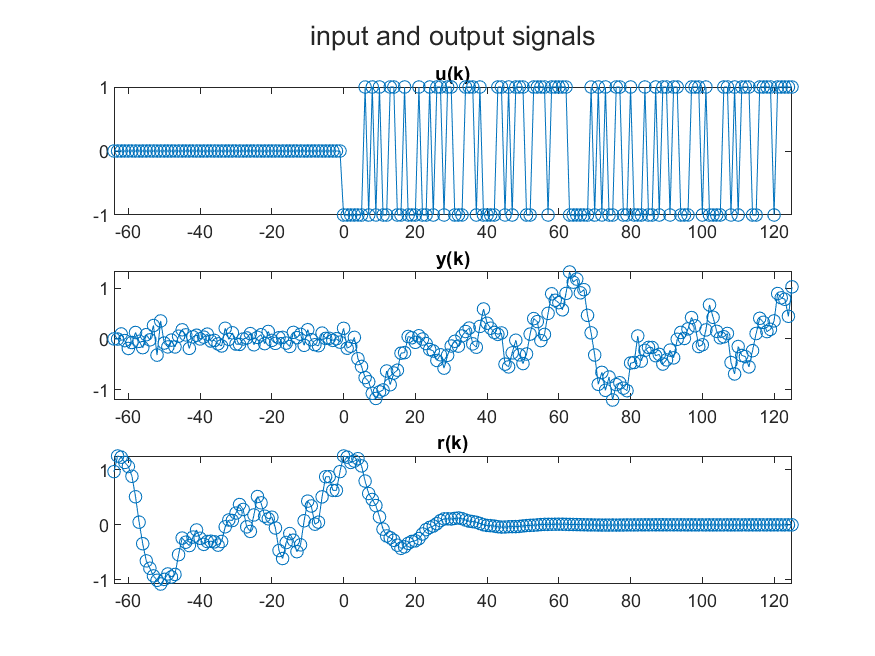
\includegraphics[width=0.8\textwidth]{"05_lect/transient-noise-time-domain.png"}
  \caption{Plot of the input $u(k)$ (top), the output $y(k)$ (middle) and transient $r(k)$ (bottom) signals, here shown only for two periods before $t=0$ and two after $t=0$.}
  \label{fig:transient-response-time-domain}
\end{figure}

What is the impact of the noise\footnote{For a periodic input signal, we have
  \begin{equation}
    \label{eq:variance-ETFE}
    \mathbb{E}\left\{\left|\hat{G}_N(e^{j\omega_n}) - G_0(e^{j\omega_n})\right|^2\right\} = \frac{\phi_v(e^{j\omega_n}) + \frac{2c}{N}}{\frac{1}{N}|U_N(e^{j\omega_n})|^2}
  \end{equation}
  the expression for $c$ is given above, and
  \begin{equation*}
    \EE{|\hat{G}(\ejwn)|^2} = |G(\ejwn)|^2 + \frac{N\phi_v(\ejwn)}{|U_N(\ejwn)|^2}.
  \end{equation*}} and the transient? What follows is my hand-waving attempt to understand the motivation to use a periodic signal. The noise signal ``behaves'' like a random input signal: disregarding the constant term in eq.~\eqref{eq:PSD-random-input-signal}, SNR remains constant for a random input signal, since
\begin{equation*}
  \frac{\EE{|V_N(\ejwn)|^2}}{\EE{|U_N(\ejwn)|^2}}
\end{equation*}
does not change for growing $N$. Instead it decreases as $\frac{1}{N}$ for periodic input signals.

\begin{figure}[h]
  \centering
  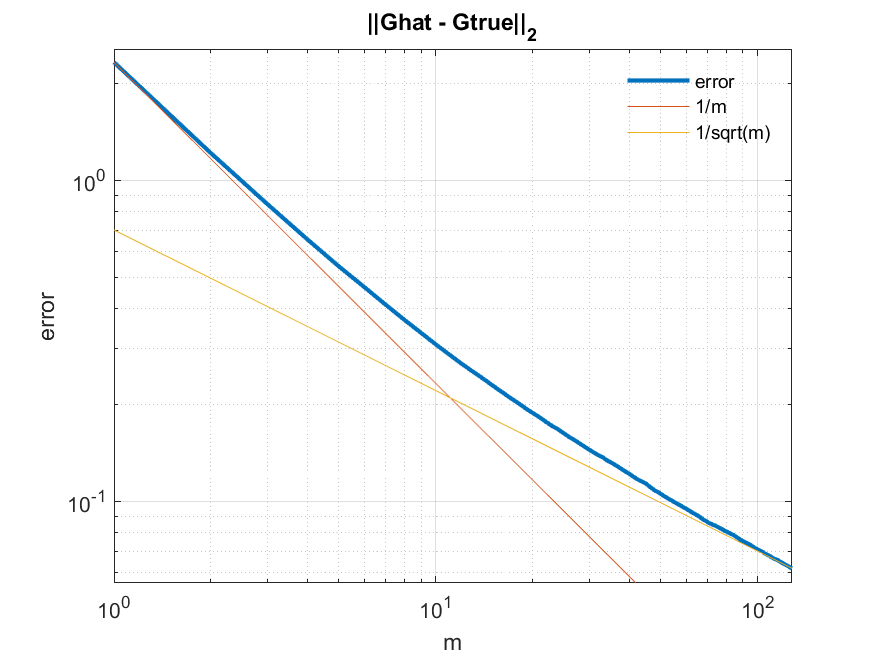
\includegraphics[width=0.8\textwidth]{"05_lect/transient-noise-convergence-avg.png"}
  \caption{Convergence of $\EE{||\hat{G}-G||_2}$ as a function of the number of periods $m$ (each of M points). The cross-over between the transient-limited convergence with dependence $\frac{1}{m}$ to noise-limited with convergence $\frac{1}{\sqrt{m}}$ is clearly visible.}
  \label{fig:transient-response-convergence}
\end{figure}

The transient instead decays exponentially: its PSD remains constant as a function of $N$ and the convergence of the SNR is $\sim\frac{1}{N}$. Fig.~\ref{fig:transient-response-time-domain} shows the output signal $y(k)$ affected by both noise and transient: the cross-over between transient-limited and noise-limited convergence is visible in Fig.~\ref{fig:transient-response-convergence}. Implementation in \texttt{05\_lect/SysID\_ETFE.m}.


%%%%%%%%%%%%%%%%%%%%%%%%%%%%%%%%%%%%%%%%%%%%%%%%%%%%%%%%%%%%
\section{Swept-Sine Identification}
\label{sec:swept-sine-identification}

The system\footnote{To my knowledge, this method is also called demodulation or lock-in detection.} is excited with the periodic input signal $u(k)=\alpha \cos(\omega_uk)$ of \emph{arbitrary} frequency $\omega_u$. The output to this excitation is
\begin{equation*}
  y(k) = \underbrace{\frac{\alpha}{2} \left[G(e^{j\omega_u})e^{+j\omega_uk} + G(e^{-j\omega_u})e^{-j\omega_uk}\right]}_\text{steady state response} + v(k) + \text{transient}.
\end{equation*}
The correlation signal
\begin{equation*}
  I(N) \doteq \frac{1}{N}\sum_{k=0}^{N-1}y(k)e^{-j\omega_u k}
\end{equation*}
converges to $\frac{\alpha}{2}G(e^{j\omega_u})$ as $N\rightarrow \infty$
\begin{align*}
  I(N) &= \frac{\alpha}{2} G(e^{j\omega_u}) + \frac{\alpha}{2N} \sum_{k=0}^{N-1} G(e^{j\omega_u})e^{-2j\omega_u k} + \text{noise and transient} \\
       &= \frac{\alpha}{2} G(e^{j\omega_u})
\end{align*}
since the non-contant components average out.

Advantages of this method:
\begin{itemize}
  \itemsep0em
\item the energy is concentrated at the frequencies of interest;
\item arbitrary frequencies can be measured and not only those determined by the Fourier transform;
\item the amplitude of $u(k)$ can easily be tuned as a function of frequency;
\item it makes it easy to avoid saturation and to tune SNR.
\end{itemize}
Disadvantages are:
\begin{itemize}
  \itemsep0em
\item a large amount of data is required;
\item significant amount of time required for experiments because single frequencies are probed sequentially;
\item some processes will not allow sinusoidal inputs.
\end{itemize}

\iffalse
  %%%%%%%%%%%%%%%%%%%%%%%%%%%%%%%%%%%%%%%%%%%%%%%%%%%%%%%%%%%%
  \section{Spectral Estimation Methods}
  \label{sec:spectral-estimation-methods}

  From eq.~\eqref{eq:freq-domain-LTI-estimator}, neglecting the transient and multiplying element-wise by $U^\star(\ejwn)$, we have
  \begin{equation*}
    \phi_{yu}(\ejwn) = G \phi_u(\ejwn) + \phi_{uv}(\ejwn)
  \end{equation*}
  the cross correlation term $\phi_{uv}(\ejwn)$ being zero if $u$ and $v$ are uncorrelated (for instance in open loop). The estimate $\hat{G}(\ejwn)$ is
  \begin{equation*}
    \hat{G}(\ejwn) = \frac{\hat{\phi}_{yu}(\ejwn)}{\hat{\phi}_u(\ejwn)}.
  \end{equation*}


  %%%%%%%%%%%%%%%%%%%%%%%%%%%%%%%%%%%%%%%%%%%%%%%%%%%%%%%%%%%%
  \subsection{ETFE vs Spectral Methods}

  It is not clear to me why would one choose spectral methods instead of ETFE.

  In the case of periodic input signals, both estimators give identical results.

  For the stochastic input signal, ``the unknown past inputs and future outputs are source of inaccuracy''. Both methods have a bias (?) but the variance for the ETFE is infinite\cite{broersen}. (What this means, I have no idea.)


  %%%%%%%%%%%%%%%%%%%%%%%%%%%%%%%%%%%%%%%%%%%%%%%%%%%%%%%%%%%%
  \section{Smoothed Correlation and Cross-Correlation}
  \label{sec:smoothed-correlations}

  The estimate $\hat{G}(e^{j\omega})$ can be smoothed using a window function $W(e^{j\omega})$:
  \begin{equation*}
    \tilde{G}_N(e^{j\omega}) = \sum_{\xi=-\frac{N}{2}+1}^{\frac{N}{2}} W_\gamma(e^{j(\xi-\omega_n)}) \alpha(e^{j\xi}) \hat{G}_N(e^{j\xi})
  \end{equation*}
  where $\alpha$ is the variance weighting of the result. The calculation is however better performed as multiplications by going back and forth with the Fourier transform.

  What is the value to use for the variance?

  Filtering is done with the Hann function or raised cosine. Its Fourier transform is real because the function is symmetric with $k$\footnote{One has
    \begin{equation*}
      X(\ejwn) = \sum_{k=0}^{N-1} x(k)[\cos(\omega_nk) - j\sin(\omega_nk)].
    \end{equation*}
  }.
\fi

%%%%%%%%%%%%%%%%%%%%%%%%%%%%%%%%%%%%%%%%%%%%%%%%%%%%%%%%%%%%
\section{Discrete Fourier Transform}
\label{sec:DFT}

The Fourier series is defined (for $M$ even) as
\begin{equation}
  \label{eq:fourier-transform}
  X(\ejwn) = \sum_{k=0}^{M-1} x(k) \emjwn[k],\hspace{2em} \omega_n = \frac{2\pi}{M}n
\end{equation}
and the inverse Fourier transform as
\begin{equation}
  \label{eq:inverse-fourier-transform}
  x(k) = \frac{1}{M}\sum_{n=0}^{M-1} X(\ejwn) \ejwn[k].
\end{equation}

%%%%%%%%%%%%%%%%%%%%%%%%%%%%%%%%%%%%%%%%%%%%%%%%%%%%%%%%%%%%
\subsection{Auto-Correlation for Periodic Signals}
\label{sec:autocorrelation-periodic}

Given the periodic signal $\{x(k)\}$, the auto-correlation function is the product of $x$ with itself delayed by $\tau$:
\begin{equation}
  \label{eq:auto-correlation}
  R_x(\tau) = \frac{1}{N}\sum_{k=0}^{N-1} x(k)x(k-\tau)
\end{equation}
and the power spectral density (PSD)\footnote{Using $\emjwn[\tau] = \emjwn[k]\cdot \emjwn[(\tau-k)]$ and eq.~\eqref{eq:auto-correlation}, one has
  \begin{align*}
    \phi_x(\ejwn) &= \frac{1}{N}\sum_{k=0}^{N-1} x(k)e^{\emjwn[k]} \left[\sum_{\tau=0}^{N-1} x(k-\tau)\emjwn[(k-\tau])\right]^\star \\
                  &= \frac{1}{N}X(\ejwn) X^\star(\ejwn)
  \end{align*}
}
\begin{equation}
  \label{eq:PSD}
  \phi_x(e^{j\omega_n}) = \sum_{\tau=0}^{N-1} R_x(\tau) e^{-i\omega_n\tau} = \frac{1}{N}|X(e^{j\omega_n})|^2.
\end{equation}

The auto-correlation has the following properties:
\begin{itemize}
\item $R_x(-\tau) = R_x^\star(\tau)$;
\item $R_x(0)\ge |R_x(\tau)|$, for all $\tau>0$.
\end{itemize}
$\phi_x(\omega)$ has the following properties:
\begin{itemize}
\item $\phi_x(\omega)$ is non-negative for all $\omega$
\item $\phi_x(\omega) = \phi_x(-\omega)$ for all real-valued $x(k)$.
\end{itemize}

%%%%%%%%%%%%%%%%%%%%%%%%%%%%%%%%%%%%%%%%%%%%%%%%%%%%%%%%%%%%
\subsection{Cross-Correlation for Periodic Signals}
\label{sec:crosscorrelation-periodic-signals}

Given the periodic signals $y(k)$ and $u(k)$, the cross-correlation function is
\begin{equation}
  \label{eq:cross-correlation}
  R_{yu}(\tau) = \frac{1}{N}\sum_{k=0}^{N-1} y(k)u(k-\tau)
\end{equation}
and the cross-spectral density
\begin{equation}
  \label{eq:cross-correlation-PSD}
  \phi_{yu}(\ejwn) = \sum_{\tau=0}^{N-1} R_{yu}(\tau) e^{-i\omega_n\tau} = \frac{1}{N}Y(\ejwn)U^\star(\ejwn).
\end{equation}


%%%%%%%%%%%%%%%%%%%%%%%%%%%%%%%%%%%%%%%%%%%%%%%%%%%%%%%%%%%%
\section{Random Signals}
\label{sec:random-signals}

We assume $e(k)\in \mathcal{N}(0,\sigma^2)$; $e(k)$ are independent and identically distributed (i.i.d.).

For random signals, the definition is in terms of the expected values: the \emph{autocorrelation} function is defined as
\begin{equation*}
  R_x(\tau) = \EE{x(k)x(k-\tau)}
\end{equation*}
and the \emph{covariance} function as
\begin{equation*}
  R_x(\tau) = \EE{\left(x(k) - \EE{x}\right)\left(x(k-\tau)-\EE{x}\right)}
\end{equation*}
It will be assumed that random signals are zero mean and the notation $R_x(\tau)$ is used for both the autocorrelation and covariance functions. The stationarity implies that the expectations only depends on the shift $\tau$.

The power spectral density is defined as the \emph{Fourier transform} of the autocovariance, $R_x(\tau)$
\begin{equation*}
  \phi_x(\ejw) = \sum_{\tau=-\infty}^\infty R_x(\tau)e^{-j\omega\tau} \hspace{1em} \omega\in[-\pi,\pi)
\end{equation*}
and the inverse transform is given by
\begin{equation*}
  R_x(\tau) = \frac{1}{2\pi}\int_{-\pi}^{+\pi} \phi_x(e^{j\omega})e^{j\omega\tau}\du \omega.
\end{equation*}

Cross-covariance and cross-correlations are similarly defined. For zero mean signals, the cross-correlation is
\begin{equation*}
  R_{yu}(\tau) = \EE{y(k)u(k-\tau)}.
\end{equation*}

The definitions for the auto- and cross-correlation given above are for infinite length signals. Since one can only collect finite-length data, one must make a sensible approximation. The difficulty arises from the fact that in system identification ``the measured output is almost always composed of the sum of a stochastic signal (from the noise) and a deterministic, or even periodic, signal from the convolution of the plant with a deterministic input signal, $u(k)$. This means that there is no obvious correct choice in deciding which autocorrelation estimation method to apply. The better method will inevitably be problem dependent.''~\cite{smith-suppl4}.

\iffalse
%%%%%%%%%%%%%%%%%%%%%%%%%%%%%%%%%%%%%%%%%%%%%%%%%%%%%%%%%%%%
\section{Periodogram}
\label{sec:periodogram}

If $\{s(t)\}$ and $\{w(t)\}$ are related by the strictly stable system $G(q)$ and the input for $t<0$ unknown but obeying $|w(t)|\le C_w$ for all $t$, one has
\begin{equation}
  \label{eq:filtered-periodogram-estimate}
  S_N(w) = G(e^{i\omega})W_N(w) + R_N(w)
\end{equation}
where
\begin{equation}
  \label{eq:estimate-transient}
  |R_N(w)| \le 2C_w\frac{C_G}{\sqrt{N}},\hspace{2em} C_G = \sum_{k=1}^\infty k|g(k)|
\end{equation}
$R_N$ is \emph{not} the transient response.

This is defined for or a random signal

\begin{equation*}
  \frac{1}{N}\left|V_N(\ejw)\right|^2
\end{equation*}
is an asymptotically unbiased estimator of the spectrum
\begin{equation*}
  \lim_{N\rightarrow \infty} \EE{\frac{1}{N} \left|V_N(\ejw)\right|^2} = \phi_v(\omega)
\end{equation*}
under the assumption that the autocorrelation decays quickly enough
\begin{equation*}
  \lim_{N\rightarrow \infty} \frac{1}{N} \sum_{\tau=-N}^N |\tau R_v(\tau)| = 0
\end{equation*}
\fi

%%% Local Variables:
%%% mode: latex
%%% TeX-master: "notes"
%%% End:

\chapter{Pulse Response Estimation}
\label{chap:time-domain}


The frequency-domain approach cannot easily deal with the transient: ignoring it leads to a biased estimate of the transfer function $\hat{G}(\ejwn)$. In the time domain approach it is easy to include the transient.

Starting\footnote{We have seen in the previous chapter that $G(e^{j\omega})$ is related to $g(\tau)$ by a Fourier transformation when the full time reponse $k\in (-\infty,+\infty)$ is available; otherwise it is only approximately true.} from eq.~\eqref{eq:linear-model-pulse}
\begin{equation*}
  y(k) \doteq \sum_{l=0}^\infty g(l)u(k-l) + v(k)
\end{equation*}
(note that here the summation\footnote{Why do we need the pass-through term?} starts from $l=0$) and expanding the relationship above gives
\begin{align*}
  y(k) &= g(0)u(k) + g(-1)u(k-1) + g(-2)u(k-2) + \ldots + v(k) \\
  y(k+1) &= g(0)u(k+1) + g(-1)u(k) + g(-2)u(k-1) + \ldots + v(k+1) \\
  y(k+2) &= \ldots
\end{align*}
which can be written in Toeplitz matrix form as
\begin{equation}
  \label{eq:TD-response-estimation-matrix}
  \begin{bmatrix}
    y(0) \\ y(1) \\ \vdots \\ y(K-1)
  \end{bmatrix} =
  \begin{bmatrix}
    u(0) & u(-1) & \ldots & u(-K+1) && \ldots \\
    u(1) & u(0) & \ldots & u(-K+2) && \ldots \\
    \vdots & & \ddots & \vdots \\
    u(K-1) & u(K-2) & & \ldots & & \hdots
  \end{bmatrix}
  \begin{bmatrix}
    g(0) \\ g(1) \\ g(2) \\ \vdots
  \end{bmatrix} +
  \begin{bmatrix}
    v(0) \\ v(1) \\ \vdots \\ v(K-1)
  \end{bmatrix}
\end{equation}
or, in matrix notation, as
\begin{equation}
  \label{eq:TD-response-estimation}
  Y = \Phi_ug + V.
\end{equation}
The existence of the estimate $\hat{g}$ and its properties depends on how $\Phi_u$ is constructed. We will consider them here.

In the following we will drop the error term $V$ to keep the notation more readable. Moreover, zero-mean Gaussian distributed error does not induce bias using least-squares estimation.

%%%%%%%%%%%%%%%%%%%%%%%%%%%%%%%%%%%%%%%%%%%%%%%%%%%%%%%%%%%%
\subsection{Estimation of Truncation Error for IIR}
\label{sec:truncation-error-estimation}

A finite impulse response (FIR) is described by a finite ($\taumax+1$) number of coefficients: that is $g(\tau) = 0$ for $\tau \ge \taumax$. $\hat{g}(\tau)$ in eq.~\eqref{eq:TD-response-estimation} can be found by least-squares.

On the contrary, for rational transfer functions (infinite impulse response, IIR) an infinite number of terms is required to describe the impulse response $g$. If the system is stable, the amplitudes of $g$ decays exponentially.

We cannot solve the least-squares problem with an infinite number of terms but the system can be truncated to a finite number of terms, since $g$ decays exponentially. This is guaranteed by the following theorem: For a strictly stable real-rational system, if all of the poles of $g$ are inside the unit-circle, then, for any $\epsilon>0$, there exists a $\taumax$ such that
\begin{equation*}
  \sum_{i=\taumax+1}^\infty |g(i)| < \epsilon
\end{equation*}
where the truncation of eq.~\eqref{eq:TD-response-estimation} gives rise to the error term
\begin{align*}
  \begin{bmatrix}
    y(0) \\ \vdots \\ y(K-1)
  \end{bmatrix} =
  \begin{bmatrix}
    u(0) & \ldots & u(-\taumax) \\
    \vdots & \ddots & \vdots \\
    u(K-1) & \ldots & u(K-\taumax-1)
  \end{bmatrix}
  \begin{bmatrix}
    g(0) \\ \vdots \\ g(\taumax)
  \end{bmatrix} +
  \begin{bmatrix}
    e(0) \\ \vdots \\ e(K-1)
  \end{bmatrix}
\end{align*}
where $Y,\ E\in \mathcal{R}^K$, $\Phi_u \in \mathcal{R}^{K\times(\taumax+1)}$ and $g \in \mathcal{R}^{\taumax+1}$. Ignoring the error makes the estimate biased: the estimate is however asymptotically unbiased as it can be made arbitrarily small by selecting a larger $\taumax$.

%%%%%%%%%%%%%%%%%%%%%%%%%%%%%%%%%%%%%%%%%%%%%%%%%%%%%%%%%%%%
\subsection{Initial Conditions: Negative Times for $g$}

The expression eq.~\eqref{eq:TD-response-estimation-matrix} requires the knowledge of the control input at negative times. If the initial conditions are not known, the corresponding terms must be discarded
\begin{equation*}
  \begin{bmatrix}
    y(\taumax) \\ \vdots \\ y(K-1)
  \end{bmatrix} =
  \begin{bmatrix}
    u(\taumax) & \ldots & u(0) \\
    \vdots & \ddots & \vdots \\
    u(K-1) & \ldots & u(K-\taumax-1)
  \end{bmatrix}
  \begin{bmatrix}
    g(0) \\ \vdots \\ g(\taumax)
  \end{bmatrix} +
  \begin{bmatrix}
    e(\taumax) \\ \vdots \\ e(K-1)
  \end{bmatrix}
\end{equation*}

%%%%%%%%%%%%%%%%%%%%%%%%%%%%%%%%%%%%%%%%%%%%%%%%%%%%%%%%%%%%
\subsection{Bad Measurements}

A bad measurement can be also easily dealt with in the time domain. Let us assume that $y(j)$ was corrupted. The problem can still be written as before with the faulty line removed:
\begin{equation*}
  \begin{bmatrix}
    % y(\taumax) \\ \vdots \\ y(j-1) \\ y(j) \\ y(j+1) \\ \vdots \\ y(K-1)
y(\taumax) \\ \vdots \\ y(j-1) \\ y(j+1) \\ \vdots \\ y(K-1)
  \end{bmatrix} =
  \begin{bmatrix}
    u(\taumax) & \ldots & & u(0) \\
    \vdots & & & \vdots \\
    u(j-1) & u(j-2) & \ldots & u(j-\taumax-2) \\
    %u(j) & u(j-1) & \ldots & u(j-\taumax-1) \\
    u(j+1) & u(j) & \ldots & u(j-\taumax) \\
    \vdots & & & \vdots \\
    u(K-1) & \ldots & & u(K-\taumax-1)
  \end{bmatrix}
  \begin{bmatrix}
    g(0) \\ g(1) \\ \vdots \\ g(\taumax)
  \end{bmatrix} +
  \begin{bmatrix}
    % e(\taumax) \\ \vdots \\ e(j-1) \\ e(j) \\ e(j+1) \\ \vdots \\ e(K-1)
e(\taumax) \\ \vdots \\ e(j-1) \\ e(j+1) \\ \vdots \\ e(K-1)
  \end{bmatrix}
\end{equation*}
and the truncation is still valid.

The problem is different if $u(j)$ were unknown: in this case all elements\footnote{This is a block of dimentions $\taumax\times \taumax$.} where $u(j)$ had an effect, must be eliminiated.

%%%%%%%%%%%%%%%%%%%%%%%%%%%%%%%%%%%%%%%%%%%%%%%%%%%%%%%%%%%%
\subsection{Uniqueness of $\hat{g}$ and Persistency of Excitation}
\label{sec:persistency-excitation}

For the solution to be unique, $\Phi_u$ needs to have full column rank. What input signals satisfy this requirement? For instance, a single sinusoidal input signal would make the matrix have rank 2 and in the frequency domain, this would determine amplitude and phase of a single frequency\footnote{In the time domain, trying to solve the rank-deficient problem results in the wrong estimate of the coefficients, see \texttt{07\_lect/persistency.jl}.}.

\begin{itemize}
\item The constant function\footnote{Prof. Smith calls is step function, but a step function makes $\Phi_u$ full matrix.} $u(k)=1$, $\forall k$ is persistently exciting of order 1;
\item a PRBS signal\footnote{This is a periodic deterministic signal with white noise-like properties. It is generated by the differential equation
    \begin{equation*}
      u(k) = \mod(A(q)u(k),2), \hspace{2em} A(q)u(k) = \sum_{i=1}^na_iu(t-i).
    \end{equation*}
    The actual period depends on the choice of $A(q)$ and for each $n$ there exists choices of $A(q)$ that give the maximum length.~\cite[Chap.~13]{ljung}. The MATLAB command is either \texttt{prbs(M,N)} or \texttt{idinput("prbs", N)}.} of period $M$ is persistently exciting of order $M$;
\item the sum of sinusoidals
  \begin{equation*}
    u(k) = \sum_{s=1}^S \alpha_s \cos(\omega_sk + \phi_s)
  \end{equation*}
  is persistently exciting of order $2S$ if $\omega_s\in (0,\pi)$. The order decreases by 1 if either one of $\omega_s = 0,\pi$ is included and by 2 if both frequencies are included. For periodic signals, $\Phi_u$ is circulant.
\end{itemize}

In class (and in \cite[Sect.~13.2]{ljung}) the uniqueness of $\hat{g}$ was discussed in terms of the rank of the auto-correlation matrix $R_u$, but discussion in Moodle indicates that checking for the singular values of $\Phi_u$ is completely equivalent.


%%%%%%%%%%%%%%%%%%%%%%%%%%%%%%%%%%%%%%%%%%%%%%%%%%%%%%%%%%%%
\subsection{Pulse Response from Cross- and Autocorrelation}
\label{sec:}

A similar relationship holds for the correlations\footnote{So was derived the expression in class: From eq.~\eqref{eq:linear-model-pulse}, we have
  \begin{align*}
    \EE{y(k)u(k-\tau)} &= \EE{\sum_{i=0}^\infty g(i)u(k-i)u(k-\tau)} + \EE{v(k)u(k-\tau)} \\
                       &= \sum_{i=0}^\infty g(i) \EE{u(k-i)u(k-\tau)} \\
                       &= \sum_{i=0}^\infty g(i) R_u(\tau-i)
  \end{align*}
}
\begin{equation*}
  R_{yu}(\tau) = g(\tau) \star R_u(\tau)
\end{equation*}
This is seen by multiplying eq.~\eqref{eq:TD-response-estimation} from the left by $\Phi_u^\top$; $R_{yu}(\tau) = \Phi_u^\top y$ and $R_u =\Phi_u^\top \Phi_u^\top$, and taking the expectations, because $\Phi_u$ is the matrix containing the shifted entries $u$.

The equivalent expression in the frequency domain was derived in Sect.~\ref{sec:spectral-estimation-methods}.

\iffalse
%%%%%%%%%%%%%%%%%%%%%%%%%%%%%%%%%%%%%%%%%%%%%%%%%%%%%%%%%%%%
\subsection{Equivalence Between Time and Frequency Domain}
\label{sec:equivalence-time-freq-domain}

Given eq.~\eqref{eq:TD-response-estimation}, the equivalence with the ETFE is established by multiplying by the Fourier transform matrix $F_y$ and $F_g$ (which may have different dimensions but are nevertheless square)
\begin{equation*}
  F_yy = F_y\Phi_uF_g^{-1}\underbrace{F_gg}_{\doteq G} + F_yv \longrightarrow \hat{G} = \left(F_y\Phi_uF_g^{-1}\right) \backslash \left(F_yy\right)
\end{equation*}
This to be equal to the standard result
\begin{equation*}
\hat{G} = F_g\cdot (\Phi_u \backslash y).
\end{equation*}


%%%%%%%%%%%%%%%%%%%%%%%%%%%%%%%%%%%%%%%%%%%%%%%%%%%%%%%%%%%%
\subsection{Slowly-Decaying Systems}
\label{sec:slowly-decaying-systems}

If $N<\taumax$, even in the periodic input case, the time response is aliased.



In the frequency domain instead, even an aliased estimate gives the correct transfer function $\hat{G}(e^{j\omega_n}) = G(e^{j\omega})|_{\omega=\omega_n}$.

%%%%%%%%%%%%%%%%%%%%%%%%%%%%%%%%%%%%%%%%%%%%%%%%%%%%%%%%%%%%
\subsection{Non-Periodic Frequency Domain Estimation}

The estimate is unbiased only when $N>\taumax$, that is when the transient has died out
\begin{equation*}
  \hat{G}(e^{j\omega_n}) = G_0(e^{j\omega_n}) + X_u^{-1}\left[V((e^{j\omega_n})) + R((e^{j\omega_n}))\right]
\end{equation*}
\fi

%%% Local Variables:
%%% mode: latex
%%% TeX-master: "notes"
%%% End:

\chapter{Error Prediction Methods and Transfer Function Models}
\label{chap:error-prediction-methods-tf}

We assume that the complete system model is given by
\begin{equation}
  \label{eq:PEM-tf-models}
  y(k) = G(z)u(k) + H(z)e(k).
\end{equation}
Prediction error-based identification methods estimate the transfer functions $G(z)$ and $H(z)$, parametrised as $G(z,\theta)$ and $H(z,\theta)$, by minimizing the objective function $J(\epsilon)$, a function of the prediction error $\epsilon(k,\theta)$
\begin{equation*}
  \epsilon(k,\theta) \doteq y(k) - \hat{y}(k,\theta).
\end{equation*}
The prediction $\hat{y}(k,\theta)$ for the time $k$ is a function of the previous measurements and inputs at $k-1,\ k-2,\ldots$ only.

%%%%%%%%%%%%%%%%%%%%%%%%%%%%%%%%%%%%%%%%%%%%%%%%%%%%%%%%%%%%
\section{Prediction}
\label{sec:prediction}

We assume that $H(z)$ is monic\footnote{Monic means that $h(0)=1$:
\begin{equation*}
  H(z) = 1 + \sum_{k=1}^\infty h(k)z^{-k}.
\end{equation*}} and stable\footnote{$H(z)$ has only poles strictly inside the unit circle.}. In this case, given the filtered noise $v(k)=H(z)e(k)$, $e(k)$ can be reconstructed from $v(k)$ as
\begin{equation}
  \label{eq:noise-reconstruction}
  e(k) = H^{-1}(z)v(k).
\end{equation}

We now seek to predict $v(k)$ given the past values up to time $k-1$: this is called the \emph{one-step ahead} estimate. Since $H(z)$ is monic, we split the filtered noise contribution into the term $e(k)$ and other terms up to time $k-1$
\begin{equation}
  \label{eq:prediction-split-filtered-noise}
  v(k) = H(z)e(k) = e(k) + \left(H(z)-1\right)e(k)
\end{equation}
The \emph{predicted} filtered noise $\hat{v}(k|k-1)$ is
\begin{equation*}
  \hat{v}(k|k-1) = (H(z)-1)e(k).
\end{equation*}
This can be intuitively understood because the error probability function distribution for $\{e\}$ has zero mean\footnote{Had the probability distribution $f_e(x)$ not had a zero mean, we would have to modify the predition according to
  \begin{equation*}
    \hat{v}(k|k-1) = \arg\max_x f_e(x - m(k-1)),\hspace{2em} m(k-1) = (H(q)-1)e(k).
  \end{equation*}}: if we were left to guess $e(k)$, we would guess $e(k)=0$. Making use of eq.~\eqref{eq:noise-reconstruction}, the one-step ahead estimate
\begin{equation}
  \label{eq:filtered-noise-one-step-prediction}
  \hat{v}(k|k-1) = \left(1-H^{-1}(z)\right)v(k)
\end{equation}
is determined only from the knowledge of the past values of $v$ up to $k-1$.

For the model of eq.~\eqref{eq:PEM-tf-models}, the one-step ahead predictor
\begin{equation}
  \label{eq:one-step-ahead-predictor-noise}
  \hat{y}(k|k-1) = G(z)u(k) + \hat{v}(k|k-1)
\end{equation}
can be rewritten with the help of the expression for $\hat{v}(k|k-1)$ as\footnote{Using $v(k) = y(k) - G(z)u(k)$
  \begin{equation*}
    \hat{y}(k|k-1) = G(z)u(k) + \left(1-H^{-1}(z)\right)\left(y(k) - G(z)u(k)\right).
  \end{equation*}
Note that $y_0(k)=G(z)u(k)$ is the evolution of the noiseless true system, so that eq.~\eqref{eq:one-step-ahead-predictor-noise} could also be written as $\hat{y}(k|k-1) = y_0(k) + \hat{v}(k|k-1)$. However we seek an expression that involves the measured outputs $y(k)$ and expressing the one-step head predictor as a function of the unknown true system is of no use to us.\label{fn:noiseless-regressor}}
\begin{equation}
  \label{eq:one-step-ahead-predictor}
  \hat{y}(k|k-1) = H^{-1}(z)G(z)u(k) + \left(1-H^{-1}(z)\right) y(k).
\end{equation}
The prediction error\footnote{Although in class the algebra was worked out, that $\epsilon(k|k-1)=e(k)$ is no surprise: $e(k)$ was the term that was discarded from $v(k)$ to compute the predicted filtered noise $\hat{v}(k|k-1)$.}
\begin{equation}
  \label{eq:one-step-ahead-predictor-error}
  \epsilon(k,|k-1) = y(k) - \hat{y}(k|k-1) = e(k)
\end{equation}
is the noise $e(k)$: the \emph{innovation} is the part of the output prediction that cannot be estimated from past measurements.

%%%%%%%%%%%%%%%%%%%%%%%%%%%%%%%%%%%%%%%%%%%%%%%%%%%%%%%%%%%%
\subsection{Example: Moving Average}

The model
\begin{equation*}
  v(k) = e(k) + ce(k-1) \rightarrow H(z) = 1+cz^{-1}
\end{equation*}
is invertible when $|c|<1$. The one-step ahead predictor eq.~\eqref{eq:filtered-noise-one-step-prediction} can be expressed in terms of the error $e(k-1)$ using eq.~\eqref{eq:one-step-ahead-predictor-error}
\begin{equation*}
  \hat{v}(k|k-1) = \left(1-H^{-1}(z)\right)H(z)e(k) = cz^{-1}e(k) =  ce(k-1)
\end{equation*}

%%%%%%%%%%%%%%%%%%%%%%%%%%%%%%%%%%%%%%%%%%%%%%%%%%%%%%%%%%%%
\section{Family of Transfer-Function Models}
\label{sec:family-tf-models}

The advantage of the transfer-function models is that they can be described by fewer parameters and that the inputs required to identify the system do not have to be persistently exciting as it is the case when one wants to identify frequency or time-response: we have seen in Sect.~\ref{} that for frequency domain methods, the order of excitation must be double the number of complex estimates of the transfer function $G(e^{j\omega_n})$ since gain and phase must be determined for each frequency; for a time response one requires the same persistency order as the number of impulse response terms.

If we control the input, this requirement is easy to satisfy. If on the other hand the data is given, this may not be the case and in these situations, one is better off looking for transfer functions/state space representations because of the reduced numbers of parameters to identify.

Prediction error-based identification methods construct the prediction error\footnote{Here we are seeking the unknown parameters $\theta$ for a known model for which we can construct the one-step ahead predictor $\hat{y}(k,\theta)$, parametrized by $\theta$. Since $\theta$ is unknown, we cannot say just yet that $\epsilon(k,\theta) = e(k)$.

  I also do not know if $\min_\theta ||\epsilon(\theta)||_2^2 = \sum_k ||e(k)||_2^2$ but I suspect this is the case when $e(k)$ is Gaussian-distributed.}
\begin{equation}
  \label{eq:prediction-error-parametrized}
  \epsilon(k,\theta) = y(k) - \hat{y}(k,\theta)
\end{equation}
from the (one-step ahead) predictor $\hat{y}(k,\theta)$ which is based on the guesses $\hat{G}(z)=G(z,\theta)$ and $\hat{H}^{-1}(z)=H^{-1}(z,\theta)$, the guesses being parametrized by $\theta$. The optimal $\theta^\star$ is the argument that minimizes the cost function $J=J(\epsilon)$
\begin{equation*}
  \theta^\star = \arg \min_\theta J(\epsilon(k,\theta)).
\end{equation*}
Typical choices for the objective functions $J(\epsilon)$ are the 2-norm $||\epsilon||_2^2$ or the maximum deviation, the $\infty$-norm $||\epsilon||_\infty$. The kind of minimization depends on how the models $G(q)$ and $H^{-1}(q)$ are parametrised: in general, the parametrization will not be linear and the optimization may not be convex. Note moreover that the minimization of $||\epsilon||_2^2$ is not equivalent to the least squres method, unless  $H(z)=1$:
\begin{equation*}
  y(k) = G(z)u(k) + e(k).
\end{equation*}

Since this approach does not require an a-priori knowlege of the system, it is also called the \emph{black-box} approach.

%%%%%%%%%%%%%%%%%%%%%%%%%%%%%%%%%%%%%%%%%%%%%%%%%%%%%%%%%%%%
\subsection{Equation Error Model Structure (ARX)}
\label{sec:ARX}

%The numerator is the moving average (MA) part, the denominator the autoregressive (AR) part, X for the exogeraneous (external) input.

The ARX model
\begin{equation}
  \label{eq:ARX-model}
  y(k) = B(z)u(k) + \left(1-A(z)\right)y(k) + e(k)
\end{equation}
is a simple input-output relationship where the error enters as a direct term: this model covers a limited set of real-world problems, for instance those where the perturbation act as a force. We take
\begin{equation*}
  A(z) = 1 + a_1z^{-1} + \ldots + a_nz^{-n},\hspace{2em} B(z) = b_1z^{-1} + \ldots + b_mz^{-m}
\end{equation*}
where $A(z)$ is monic and $B(z)$ does not contain a constant term, \textit{i.e.} the model has no feed-through. It corresponds to the model of eq.~\eqref{eq:PEM-tf-models} with
\begin{equation*}
  G(z) = \frac{B(z)}{A(z)},\hspace{2em}H(z) = \frac{1}{A(z)}.
\end{equation*}
and generates the one-step ahead predictor
\begin{equation}
  \label{eq:one-step-ahead-ARX}
  \hat{y}(k|k-1) = \left(1-A(z)\right)y(k) + B(z)u(k)
\end{equation}
either by plugging $G(z)$ and $H^{-1}(z)$ in eq.~\eqref{eq:one-step-ahead-predictor} or by using the result of eq.~\eqref{eq:one-step-ahead-predictor-error} in eq.~\eqref{eq:ARX-model}.

We now seek the estimates $\hat{B}(z,\theta)$ and $\hat{A}(z,\theta)$ parametrized by the \emph{parameter vector} $\theta$ which contains the unknown coefficients of the polynomials $A(z)$ and $B(z)$
\begin{equation*}
  \theta =
  \begin{bmatrix}
    a_1 & \ldots & a_n & b_1 & \ldots & b_m
  \end{bmatrix}^\top
\end{equation*}
This generates the one-step ahead predictor
\begin{equation*}
  \hat{y}(k,\theta) = \left(1-\hat{A}(z,\theta)\right)y(k) + \hat{B}(z)u(k).
\end{equation*}
that can be written in linear form
\begin{equation*}
  \varphi^\top(k) =
  \begin{bmatrix}
    -y(k-1) & \ldots & -y(k-n) & u(k-1) & \ldots & u(k-m)
  \end{bmatrix}.
\end{equation*}
using the \emph{regressor vector} $\varphi(k)$ that contains the outputs and inputs.

$\theta$ is found by minimization of the prediction error $\epsilon(k,\theta) = y(k) - \hat{y}(k,\theta)$: when $\theta$ is the true parameter vector $\theta_0$, then $\epsilon(k,\theta_0)=e(k)$. Generally, one minimizes the 2--norm $||\epsilon(k,\theta)||_2^2$: this  is solved in MATLAB by
\begin{equation}
  \label{eq:ARX-solution}
  %\Phi\hat{\theta} = Y\rightarrow
  \hat{\theta} = \Phi \backslash Y,\hspace{2em} \Phi \doteq
  \begin{bmatrix}
    \varphi^\top(1) \\ \varphi^\top(2) \\ \ldots \\ \varphi^\top(N)
  \end{bmatrix}, \hspace{1em} Y \doteq
  \begin{bmatrix}
    y(1) \\ y(2) \\ \ldots \\ y(N)
  \end{bmatrix}
\end{equation}
The first element of the regressor is $\varphi(1)$ that depends on the past indeces up to $k=0$: these are the initial conditions. They are usually specified by the system being at rest; otherwise, one must drop a certain amount of entries (how many exactly?)

%%%%%%%%%%%%%%%%%%%%%%%%%%%%%%%%%%%%%%%%%%%%%%%%%%%%%%%%%%%%
\subsection{ARX: Estimate Bias}
\label{sec:estimate-bias-ARX}

The numerical example in class (slides 9-30 to 9--34) confused me. In the first situation we have
\begin{equation*}
  \frac{B(z)}{A(z)} = \frac{bz^{-1}}{1 + az^{-1}}, \hspace{2em} H(z)=1.
\end{equation*}
The one-step ahead predictor is
\begin{equation*}
  \hat{y}(k|k-1) = y(k) - e(k) = \frac{B(z)}{A(z)}u(k) = \varphi_0^\top(k)\theta_0
\end{equation*}
is nothing else than the evolution of the true system. The regressor $\Phi_0$ must be constructed from the true $y_0(k) = \frac{B(z)}{A(z)}u(k)$: using instead the measured $y(k)$ gives the bias of slide 9--30. (See also discussion in Sect.~\ref{sec:estimation-bias}.)

\begin{figure}[h]
  \centering
  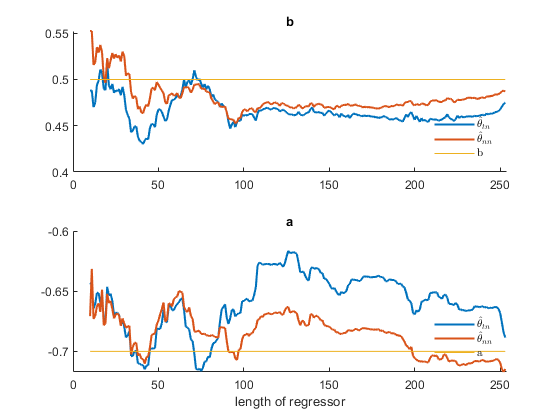
\includegraphics[width=0.8\textwidth]{09_lect/ARX-bias.png}
  \caption{Comparison of estimates with true and noisy regressors and data for a PRBS input signal with $O=7$ and $N=127$. The estimates start from a minimum regressor length of $10$. The code is in \texttt{09\_lect/SysID\_ARX.m}.}
  \label{fig:estimate-bias-ARX}
\end{figure}

In the second situation, we take the noise to be $H(z) = \frac{1}{A(z)}$. In Fig.~\ref{fig:estimate-bias-ARX} I compare the solutions of the least square problems
\begin{equation*}
  \hat{\theta}_{tn} \doteq \Phi_0\backslash Y,\hspace{2em} \hat{\theta}_{nn} \doteq \Phi\backslash Y
\end{equation*}
as a function of the number of elements in the regressor, just as it was done in class for the first problem. Only by looking at the graph, it is not possible to tell whether an estimate is biased, but repeating the experiment reveals that neither $\hat{\theta}_{nn}$ (as expected) nor $\hat{\theta}_{tn}$ (perhaps unexpectedly) are biased.

The explanation is the following: the (noisy) system's evolution is
\begin{equation*}
  y(k) = (1-A(z))y(k) + B(z)u(k) + e(k) = \varphi^\top(k)\theta_0 + e(k)
\end{equation*}
and I \emph{pick}\footnote{The word ``pick'' is emphasized: it is the true predictor but, at least for ARX, it seems to me that the most convenient predictor for the solution of the least-squares is whatever regressor the true system uses.} the one-step ahead predictor to be $\hat{y}(k,\theta) = \varphi^\top(k)\theta$. Their difference
\begin{equation*}
  y(k)-\hat{y}(k,\theta) = \varphi^\top(k)(\theta_0-\theta) + e(k)
\end{equation*}
is minimized when $\theta=\theta_0$ since $e(k)$ is Gaussian distributed: this is the case $\Phi\backslash Y$. On the other hand, we can also write
\begin{equation*}
  y(k) = y_0(k) + \frac{1}{A(z)}e(k) = \varphi_0^\top(k)\theta_0 + \frac{1}{A(z)}e(k)
\end{equation*}
and I \emph{choose}\footnote{ As mentioned already in footnote~\ref{fn:noiseless-regressor}, the noiseless regressor $\Phi_0$ cannot be constructed from the noisy data unless (I think) $H(z)=1$ when $\hat{y}(k|k-1)=y_0(k)$.} the predictor to be $\hat{y}(k,\theta) = \varphi_0^\top(k)\theta$. Their difference
\begin{equation*}
  y(k) - \varphi_0^\top(k)\theta = \varphi_0^\top(k)(\theta_0-\theta) + \frac{1}{A(z)}e(k)
\end{equation*}
is also minimized when $\theta=\theta_0$ since $\frac{1}{A(z)}e(k)$ has Gaussian distribution (although it is now correlated). This means
\begin{equation*}
  \EE{\Phi\backslash Y} = \EE{\Phi_0\backslash Y} = \theta_0
\end{equation*}
are both unbiased.

%%%%%%%%%%%%%%%%%%%%%%%%%%%%%%%%%%%%%%%%%%%%%%%%%%%%%%%%%%%%
\subsection{ARMAX Model Structure}
\label{sec:ARMAX}

The ARX model structure is not very flexible with regards to the noise model requiring it to have the particular structure $\frac{1}{A(z)}$. The ARMAX transfer function model partially relaxes this: it has the form
\begin{equation}
  \label{eq:ARMAX-model}
  A(z)y(k) = B(z)u(k) + C(z)e(k)
\end{equation}
where $A(z)$ and $B(z)$ are as in ARX and $C(z)$ is monic. It corresponds to the model of eq.~\eqref{eq:PEM-tf-models} with
\begin{equation*}
  G(z) = \frac{B(z)}{A(z)},\hspace{2em} H(z) = \frac{C(z)}{A(z)}
\end{equation*}
and with the one-step ahead predictor\footnote{In alternative to plugging the expressions for $G(z)$ and $H^{-1}(z)$ into eq.~\eqref{eq:one-step-ahead-predictor}, the one-step ahead predictor can be equally easily obtained from eq.~\eqref{eq:ARMAX-model} and eq.~\eqref{eq:one-step-ahead-predictor-error}:
  \begin{align*}
    \hat{y}(k|k-1) &= y(k) - e(k) \\
                   &=\left(1-A(z)\right)y(k) + B(z)u(k) + \left(C(z)-1\right)e(k) \\
                   &= \left(1-A(z)\right)y(k) + B(z)u(k) + \left(C(z)-1\right)\left(y(k)-\hat{y}(k|k-1)\right).
  \end{align*}
  This operation only makes sense when $H(z)$ is stably invertible though: at least $C(z)$ cannot have unstable zeros.

  Consistency check: this expression reduces to ARX one-step ahead predictor eq.~\eqref{eq:one-step-ahead-ARX} when $C(z)=1$.}
\begin{equation}
  \label{eq:one-step-ahead-ARMAX}
  \hat{y}(k|k-1) = (1-A(z))y(k) + B(z)u(k) + (C(z)-1)\left(y(k)-\hat{y}(k|k-1)\right)
\end{equation}

Introducing the regression vector
\begin{equation*}
  \varphi^\top(k,\theta) =
  \begin{bmatrix}
    -y(k-1) & \ldots & u(k-1) & \ldots & \epsilon(k-1,\theta) & \ldots
  \end{bmatrix}
\end{equation*}
eq.~\eqref{eq:one-step-ahead-ARMAX} induces the pseudolinear regression
\begin{equation}
  \label{eq:pseudolinear-regression-ARMAX}
  \hat{y}(k,\theta) = \varphi^\top(k,\theta) \theta
\end{equation}
the equation is non-linear because the unknown appears also in the regressor $\varphi^\top(k,\theta)$.

Since the regressor is pseudolinear, using non-linear least-squares to estimate $\theta$ will result in a biased estimate (why exactly?).

%%%%%%%%%%%%%%%%%%%%%%%%%%%%%%%%%%%%%%%%%%%%%%%%%%%%%%%%%%%%
\subsection{Constrained Minimization}
\label{sec:ARMAX-minimization}

Using eq.~\eqref{eq:pseudolinear-regression-ARMAX} and eq.~\eqref{eq:prediction-error-parametrized}, we have that $y(k) = \varphi^\top(k,\theta) \theta + \epsilon(k,\theta)$: this is used as the constraint in the optimization-based algorithm for the solution to the ARMAX problem:
\begin{equation*}
  \begin{aligned}
    \min_{\theta,\epsilon}\ & ||\epsilon||_2^2 \\
    \textrm{subject to } & Y = \Phi(\epsilon)\theta + \epsilon
  \end{aligned}.
\end{equation*}

% MATLAB code? Numerical example shows overfitting

\iffalse
\begin{lstlisting}[
style=Matlab-editor,
basicstyle=\mlttfamily\small]

PhiTyu = [toeplitz(u(1:end-1), [u(1); 0]), ...
    toeplitz(-y(1:end-1), [-y(1); 0])];

[x,fval] = fmincon(@(x) ARMAXobjective(x),x0, ...
    [],[],[],[],[],[],@(x)ARMAXconstraint(x,y,PhiTyu));

function f = ARMAXobjective(x) % x = [theta; e]
f = norm(x(7:end), 2);
end

function [c,ceq] = ARMAXconstraint(x,y,PhiTyu)
theta = x(1:6);
e = x(7:end);
PhiTe = toeplitz(e(1:end-1), [e(1); 0]);
ceq = y(2:end) - [PhiTyu, PhiTe] * theta - e(2:end);
c = [];
end
\end{lstlisting}
\fi

A reference implementation is in \texttt{11\_lect/SysID\_ARMAX.m}.

%%%%%%%%%%%%%%%%%%%%%%%%%%%%%%%%%%%%%%%%%%%%%%%%%%%%%%%%%%%%
\subsection{General Family of Model Structures}
\label{sec:general-family-models}

The most general family of model structure is~\cite[Sect.~4]{ljung}
\begin{equation}
  \label{eq:general-family-models}
  A(z)y(k) = \frac{B(z)}{F(z)}u(k) + \frac{C(z)}{D(z)}e(k)
\end{equation}
Some of the common cases that we have seen so far are summarized in Table~\ref{tbl:black-box-models}.

\begin{table}[h]
  \centering
  \begin{tabular}[h]{ll}
    \toprule
    Polynomials & Name of Model Structure \\
    \midrule
    B & FIR \\
    A\ B & ARX \\
    A\ B\ C & ARMAX \\
    A\ B\ C\ D & ARARMAX \\
    B\ F\ C\ D & Box-Jenkins \\
    \bottomrule
  \end{tabular}
  \caption{Some common black-box SISO models using the polynomials of eq.~\eqref{eq:general-family-models}.}
  \label{tbl:black-box-models}
\end{table}

%%%%%%%%%%%%%%%%%%%%%%%%%%%%%%%%%%%%%%%%%%%%%%%%%%%%%%%%%%%%
\subsection{Known Noise Model (with AR Noise Dynamics)}
\label{sec:known-noise-model}

This was partially addressed in the exercises. If the noise model $L(z)$ is known
\begin{equation*}
  y(k) = \frac{B(z)}{A(z)}u(k) + \frac{L(z)}{A(z)}e(k)
\end{equation*}
and provided $L(z)$ is stably invertible, by letting $y_L\doteq L^{-1}y$ and $u_L\doteq L^{-1}u$, one obtains the standard ARX form
\begin{align*}
  y_L(k) &= \frac{B(z)}{A(z)}u_L(k) + \frac{1}{A(z)}e(k) \\
  %y_L &= \frac{B}{A}u_L + \frac{1}{A}e \\
% \hat{y}_L(k|k-1) &= \underbrace{\left(1-A(z)\right)y_L(k) + B(z)u_L(k)}_{\Phi_L\theta_0}
\hat{y}_L(k|k-1) &= \underbrace{\left(1-A\right)y_L + Bu_L}_{\Phi_L\theta_0}
\end{align*}
for which, as usual, $y_L(k) - \hat{y}_L(k|k-1) = e(k)$. The estimate for $A(k,\theta)$, $B(k,\theta)$ is obtained by least-squares minimization of the prediction error $y_L(k) - \hat{y}_L(k,\theta)$. In terms of $y(k)$, the prediction error
\begin{equation*}
  y(k) - L(z)\hat{y}_L(k|k-1) = L(z)e(k)
\end{equation*}
is the filtered error $L(z)e(k)$ but since filtered Gaussian noise is still Gaussian, the estimate remains unbiased. Note that
\begin{equation*}
  L(z)\hat{y}_L(k|k-1) \neq \hat{y}(k|k-1)
\end{equation*}
is \emph{not} the one-step ahead prediction for $y(k)$, because we expect the difference to be $e(k)$.

If one were to use eq.~\eqref{eq:one-step-ahead-predictor} to compute the one-step ahead predictor for which the prediction error is $e(k)$, one would obtain the linear expression $\Phi_L\theta_0$ plus an offset term
\begin{align*}
  \hat{y}(k|k-1) &= \frac{B(z)}{L(z)}u(k) + \frac{L(z)-A(z)}{L(z)}y(k) \\
                 %&= B(z)u_L(k) + \left(L(z)-A(z)\right)y_L(k) \\
                 %&= \underbrace{\left(1-A(z)\right)y_L(k) + B(z)u_L(k)}_{\Phi_L\theta_0} + \left(L(z)-1\right)y_L(k)
                 &= Bu_L + \left(L-A\right)y_L \\
                 &= \underbrace{\left(1-A\right)y_L + Bu_L}_{\Phi_L\theta_0} + \left(L-1\right)y_L
\end{align*}
which must be subtracted from $y(k)$.


%%% Local Variables:
%%% mode: latex
%%% TeX-master: "notes"
%%% End:

\chapter{Closed-Loop Identification}
\label{chap:closed-loop-identification}


There are reasons to use system identification in closed loop:
\begin{itemize}
\item an unstable system must be operated in closed-loop. A simple controller stabilizes the system, but one may want to have a better model to improve the performance or because the system may change with time;
\item operational constraints may require closed-loop: \textit{e.g.} an operational industrial process cannot run in open loop for the purpose of identification because the specs on the final product must still be met;
\item closed-loop controller maintains the system close to the operating point of interest (the system may be non-linear and closed loop linearizes it);
\item this emphasizes plant dynamics close to the cross-over frequency range by removing a possibly large-scale zero-frequency response which is easy to control with a slow controller.
\end{itemize}
In open-loop, system identification can be performed in the frequency and time domain. In frequency domain for instance the estimate
\begin{equation*}
  \hat{G}(\ejwn) = \frac{\hat{Y}}{\hat{U}}
\end{equation*}
with
\begin{align*}
  \textrm{bias:}\hspace{1em} & \EE{\hat{G}(\ejwn) - G(\ejwn)} \longrightarrow 0 as  \\
  \textrm{variance:}\hspace{1em} & \EE{|\hat{G}(\ejwn) - G(\ejwn)|^2} \longrightarrow \frac{\phi_v(\ejwn)}{\phi_u(\ejwn)}
\end{align*}
as $N\rightarrow 0$. In closed-loop, the identification results may not be as good.

%%%%%%%%%%%%%%%%%%%%%%%%%%%%%%%%%%%%%%%%%%%%%%%%%%%%%%%%%%%%
\section{Methods for Closed-Loop Identification}
\label{sec:methods-closed-loop}


The fundamental assumption to derive the results until now was that control input $u$ and noise $e$ were uncorrelated: $\phi_{ue}(\ejw) = 0$. In closed-loop this is no longer the case: the noise on the output is seen at the input through the feedback loop.

For identification, we assume
\begin{itemize}
\item a generalized reference $r(k) = r_2(k) + C(z)r_1(k)$;
\item $y(k)$ and $u(k)$ are available;
\item $C(z)$ stabilize the system and makes it internally stable: that is, all transfer functions (the Gang of Four)
\begin{equation*}
  \frac{GC}{1+GC},\ \frac{G}{1+GC},\ \frac{C}{1+GC},\ \frac{1}{1+GC}
\end{equation*}
are stable.
\end{itemize}

There are four main methods for closed-loop identification:
\begin{itemize}
\item direct methods;
\item indirect methods;
\item joint input-output methods;
\item dual-Youla parametrization.
\end{itemize}

%%%%%%%%%%%%%%%%%%%%%%%%%%%%%%%%%%%%%%%%%%%%%%%%%%%%%%%%%%%%
\subsection{Direct Methods}
\label{sec:direct-methods}

It applies the basic prediction error method Sect. in a straightforward manner: use the output $y$ of the process and the input $u$ in the same way as for open loop operation, ignoring any possible feedback, and not using the reference signal $r$. The method works regardless of the complexity of the regulator and requires no knowledge about the character of the feedback~\cite{ljung}.

The closed loop transfer functions are
\begin{equation*}
  %\label{eq:closed-loop-tf}
  \begin{aligned}
    y &= SGr + Sv \\
    u &= Sr - SCv
  \end{aligned}
\end{equation*}
where $S(\ejw)$ is the stable sensitivity function for the closed loop system
\begin{equation*}
  S(\ejw) = \frac{1}{1+C(\ejw)G_0(\ejw)}.
\end{equation*}
Using spectral analysis\footnote{One more time, I have the impression that the result could have equally well been expressed in terms of ETFE without the need of using the correlations.}, and assuming $\phi_{rv}=0$, we have that
\begin{align*}
  \hat{\phi}_{yu}(\ejw) &= |S|^2G\phi_r - |S|^2\bar{C}\phi_v \\
  \hat{\phi}_u(\ejw) &= |S|^2\phi_r - |S|^2|C|^2\phi_v.
\end{align*}
The direct method estimates $G$ directly from $\hat{\phi}_{yu}$ and $\hat{\phi}_u$:
\begin{equation*}
  \hat{G}(\ejw) = \frac{\hat{\phi}_{yu}(\ejw)}{\hat{\phi}_u(\ejw)} = \frac{G\phi_r - \bar{C}\phi_v}{\phi_r - |C|^2\phi_v}
\end{equation*}
which converges to $G$ when the contribution from the reference signal dominates the noise.

The simplification of $|S|^2$ hides the fact that for frequencies for which $|S|^2\sim 0$, \textit{e.g.} when the loop transfer function $C(z)G(z)$ contains an integrator $\sim s^{-1}$, the measured signals $\hat{\phi}_{yu}$ and $\hat{\phi}_u$ are zero. On the other hand, in every practical control system with tracking, $S$ has a bump at around the closed loop BW (is this true?): those are the frequencies that get emphasized and are relevant for the stability.

%%%%%%%%%%%%%%%%%%%%%%%%%%%%%%%%%%%%%%%%%%%%%%%%%%%%%%%%%%%%
\subsection{Indirect Methods}
\label{sec:indirect-methods}

It identifies the closed loop transfer function\footnote{In class the method was described in the frequency domain; Ljung does it in the time-domain.} $T_{yr}(z)$ from reference input $r(k)$ to output $y(k)$, and retrieve from that the open loop system, making use of the knowledge of the regulator $C(z)$~\cite{ljung}.

Given the closed loop system
\begin{equation*}
  y(k) = T_{yr}(z)r(k) + v_{cl}(k) = \frac{G(z)}{1+G(z)C(z)}r(k) + \frac{1}{1+G(z)C(z)}v(k)
\end{equation*}
the open loop transfer function estimate $\hat{G}(z)$ is retrieved from
\begin{equation*}
  T_{yr}(z) = \frac{\hat{G}(z)}{1+\hat{G}(z)C(z)}.
\end{equation*}
Only the estimate $T_{yr}(z)$ is asymptotically unbiased because the reference $r$ is known; $\hat{G}$ (probably) does not converge to $G$ because the transformation is non-linear which does not preserve the mean.

The advantage with the indirect method is that any idenfication method can be applied to estimate $T_{yr}(z)$. On the other hand, any error in the knowledge of $C(z)$ will be reflected in $\hat{G}(z)$.

%%%%%%%%%%%%%%%%%%%%%%%%%%%%%%%%%%%%%%%%%%%%%%%%%%%%%%%%%%%%
\subsection{Joint Input-Output Methods}
\label{sec:joint-input-output-methods}

It relies on independent measurements of $y$ and $u$
\begin{equation*}
  \begin{aligned}
    y &= SGr + Sv = T_{yr}r + Sv \\
    u &= Sr - SCv = T_{ur}r - SCv
  \end{aligned}
\end{equation*}
so that their noise is uncorrelated, to estimate (asymptotically unbiased) $\hat{T}_{yr}(z)$ and $\hat{T}_{ur}(z)$; their noise is also uncorrelated. Since
\begin{equation*}
  \frac{T_{yr}}{T_{ur}} = \frac{SG}{S} = G
\end{equation*}
the estimate for $\hat{G}$ follows as the ratio
\begin{equation*}
  \hat{G}(z) = \frac{\hat{T}_{yr}(z)}{\hat{T}_{ur}(z)}.
\end{equation*}
As before, since the estimated spectra are weighted by $S$ or $S(z)C(z)$ and $S$ may become small, some frequencies may not be reliably resolved when taking the ratio. Key points:
\begin{itemize}
\item $\hat{G}$ may not be unbiased (unless the input signal is periodic?);
\item the noise enters in a complicated manner;
\item one key advantage: $C$ does not need to be known.
\end{itemize}

This method can be seen as the specific case of a more general framework~\cite[Sect.~13.5]{ljung} that works also for large interconnected systems, where there is no measurable reference $r$ (\textit{e.g.} large interconnected systems where it is also not possible to model the controller). The model is
\begin{equation*}
  \begin{aligned}
    y &= GS(r+w) + Sv= G_{cl}r + v_1 \\
    u &= S(r+w) - CSv = T_{ru}r + v_2
  \end{aligned}
\end{equation*}
When including the correlations between $v_1 = Sv + GSw$ and $v_2 = -CSv + Sw$ gives
\begin{equation*}
  \begin{bmatrix}
    y \\ u
  \end{bmatrix} = \mathcal{G}r + \mathcal{H}v.
\end{equation*}
When instead the correlations are ignored gives the method described at the beginning of this section.

%%%%%%%%%%%%%%%%%%%%%%%%%%%%%%%%%%%%%%%%%%%%%%%%%%%%%%%%%%%%
\subsection{Dual-Youla Methods}
\label{sec:dual-youla-methods}

It relies on coprime factorization of transfer functions
\begin{equation*}
  G(s) = \frac{N_0(s)}{D_0(s)}
\end{equation*}
where $N_0(s)$ and $D_0(s)$ are stable and have no common zeros.

The Bezout identity states that $N_0(s)$ and $D_0(s)$ are coprime iff there exists $U$ and $V$ such that
\begin{equation*}
  UN_0 + VD_0 = I.
\end{equation*}
A coprime factorization is ``normalised'' if
\begin{equation*}
  D_0^*D_0 + N_0^*N_0 = I.
\end{equation*}
The MATLAB command is \texttt{sncfbal}.

The Youla parametrisation is a way of parametrize all stable controllers: given a controller $C_0=\frac{X_0}{Y_0}$ with $X_0$, $Y_0$ a coprime factorization and stable (an integral controller would not work) which stabilizes $G_0$, all controllers $C$ stabilizing $G_0 = N_0/D_0$ have the form
\begin{equation*}
  C_Q = \frac{X_0+QD_0}{Y_0-QN_0}
\end{equation*}
with $Q$ stable.

The dual Youla parametrization method takes the opposite route: given the known controller $C$ that stabilizes the system, the plant $G$ must be one of those that can be stabilized by $C$. The problem can be therefore formulated as a search on stable\footnote{In class we used $R$ as the stable search transfer function, but $R$ was used for the transient in frequency-domain and $r$ for the closed-loop reference in time-domain. To avoid confusion, I use $Q$.} $Q$: find the estimate $\hat{G}$ from the set of all plants stabilized by $C(s)$. %$\hat{G}$ is automatically

We model the open-loop system as
\begin{equation}
  \label{eq:dual-youla-model-open-loop}
  y(k) = \frac{N}{D}u(k) + \frac{F}{D}e(k) \rightarrow Dy = Nu + Fe
\end{equation}
with $F$ stable and stably invertible\footnote{I guess this means all zeros and poles strictly inside the unit circle.}. Let $C_0=\frac{X_0}{Y_0}$ any stabiling controller: the choice of $X_0$, $Y_0$ makes a difference only from a numerical point of view. The parametrization gives
\begin{equation*}
  G_Q = \frac{N}{D} = \frac{N_0+QY_0}{D_0-QX_0},\hspace{2em} H_{Q,F} = \frac{F}{D} = \frac{F}{D_0-QX_0}
\end{equation*}
The equivalent open loop identification experiment is obtained by rewriting eq.~\ref{eq:dual-youla-model-open-loop} as
\begin{equation*}
  (D_0-QX_0)y = (N_0+QY_0)u + Fe %\rightarrow D_0y-N_0u = Q(X_0y+Y_0u) + Fe
\end{equation*}
or equivalently, after rearranging the terms, as
\begin{equation*}
  \begin{aligned}
    \beta &\doteq D_0y-N_0u \\
    \alpha &\doteq X_0y+Y_0u = X_0\left(y + \frac{Y_0}{X_0}u\right) = X_0r \\
    \beta &= Q\alpha + Fe.
  \end{aligned}
\end{equation*}
where the quantity $r = y + \frac{Y_0}{X_0}u$ is the reference signal $r$.

As it is written, this is an open-loop since there is no feedback between $\beta$ and $\alpha$. The procedure for the dual-Youla method is the following: given a stabilizing controller $C_0$
\begin{itemize}
\item factorise $C_0 = X_0/Y_0$;
\item choose the excitation $r$;
\item run closed-loop experiments with $C_0$, measuring $y$ and $u$.
\item choose an initial model, $G_0 = \frac{N_0}{D_0}$ (must be stabilised by $C_0$);
\item filter the measurements, $\beta = D_0y - N_0u$ (time or frequency domain);
\item filter the excitation $\alpha = Y_0r$;
\item estimate $\hat{Q}$ and $\hat{F}$ from $\beta = Q\alpha + Fe$;
\item calculate the plant estimate $\hat{G} = (N_0+\hat{Q}Y_0)(D_0 - \hat{Q}X_0)$.
\end{itemize}

\iffalse
%%%%%%%%%%%%%%%%%%%%%%%%%%%%%%%%%%%%%%%%%%%%%%%%%%%%%%%%%%%%
\section{Ratio of Distributions}
\label{sec:ratios}

if no reference the estimate is the controller. Taking more data does not help (why?)

Ratio distributions

What is the problem with the statistics?

X and Y are stochastics independent and uncorrlated variables: what is $X/Y$? The proble is because $\EE{\frac{1}{Y}} \neq \frac{1}{\EE{Y}}$

The Cauchy distribution is
\begin{equation*}
  \frac{1}{\pi}
\end{equation*}
but it does not have the mean value $\int z f(z)\du z$

Bias should not be used but rather consistency when there is a non-linear transofrmation

When taking more data, the probability of hitting the zero at the denominator is small. The right question is what is the probabilty of making an error larger than a specified $\epsilon$.
\fi

%%% Local Variables:
%%% mode: latex
%%% TeX-master: "notes"
%%% End:

\chapter{State-Space}
\label{chap:state-space}



\printbibliography

\end{document}

%%% Local Variables:
%%% mode: latex
%%% TeX-master: t
%%% End:
